\documentclass[14pt,a4paper]{scrartcl}
%too many packeges
\usepackage[utf8]{inputenc}
\usepackage[english]{babel}
\usepackage{indentfirst}
\usepackage{misccorr}
\usepackage{apacite}
\usepackage{graphicx}
\usepackage[section]{placeins}
\usepackage{float}
\usepackage{tabularx}
\usepackage{color}
\usepackage{fancyhdr}
\usepackage{times}
\usepackage{gensymb}
\usepackage{verbatim}
\usepackage{mathtools}
\usepackage{titlesec}
\usepackage{url}
\usepackage[T1]{fontenc} 
\usepackage{sectsty}
\usepackage{natbib}
\usepackage{makecell}
\usepackage{dsfont}
\usepackage[labelsep=period]{caption}
\usepackage{subcaption}
\usepackage{setspace}
\usepackage{titletoc}
\usepackage{mathrsfs}
\usepackage{circuitikz}
\usepackage{tcolorbox}
\usepackage{lipsum}
\usepackage{mathptmx}
\usepackage[font=small]{caption} % hypcap is true by default so [hypcap=true] is optional in \usepackage[hypcap=true]{caption}
\usepackage[nottoc,notlot,notlof]{tocbibind}
\definecolor{mygray}{gray}{0.4}
\usepackage[top=2.5cm,bottom=2.5cm,right=2.5cm,left=2.5cm,bindingoffset=0cm]{geometry}
\usepackage[colorlinks=true, a4paper=true, pdfstartview=FitV,
linkcolor=black, citecolor=mygray, urlcolor=black]{hyperref}

\DeclareMathOperator*{\argmax}{arg\,max}

%formating routine
\titleformat{\subsection}[block]{\bfseries{\hspace{2em}}}{\thesubsection}{1em}{}
\titleformat{\subsubsection}[block]{\bfseries{\hspace{3em}}}{\thesubsubsection}{1cm}{}
\newcommand{\sectionbreak}{\pagebreak}
\sectionfont{\centering}
\renewcommand{\baselinestretch}{1.5}
\captionsetup{compatibility=false}
\setlength{\parindent}{0.5in}
\setlength{\parskip}{6pt}
\graphicspath{ {images/} }
\linespread{1.25}
\pdfcompresslevel=9

%Macros for numeration
\makeatletter
\renewcommand{\@seccntformat}[1]{%
  \ifcsname prefix@#1\endcsname
    \csname prefix@#1\endcsname
  \else
    \csname the#1\endcsname\quad
  \fi}
\newcommand\prefix@section{Chapter \thesection. }
\makeatother
%Hack for prefixes in toc
\titlecontents{section}[3.5em]{\medskip\bfseries}
{\contentslabel[\color{black}Chapter \thecontentslabel]{4.5em}\enspace}
{\hskip-3em}
{\titlerule*[1.2pc]{.}\contentspage}

\newcommand{\norm}[1]{\left\lVert#1\right\rVert}
\begin{document}

  \begin{titlepage}
      \begin{center}
        \large
        \textbf{The Government of the Russian Federation}
        
        \textbf{Federal State Autonomous Educational Institution\\of Higher Professional Education}
        \vspace{0.25cm}
        
       \textbf{National Research University – Higher School of Economics}
       \vspace{0.25cm}

        Faculty of Computer Sciences
        \\Master's programme in Data Analysis in Biology and Medicine\\[1cm]
        
        \textbf{Graduate Coursework}
        \\[0.5cm]
        \textbf{\guillemotleft The Role Of L-Lactate In Sleep And Torpor Regulation \guillemotright}
        \vfill
         
      \end{center}

  \newlength{\ML}
  \hfill\begin{minipage}{0.4\textwidth}
    \textbf{Student group ADBM2018}\\[0.3cm]
    \underline{Minkov V.\,A.} \\
    \scriptsize{Last name, First name, Middle name}\\\\
    \large
    \underline{\hspace{7cm}}
    \scriptsize{Signature}\\
      \end{minipage}%


  \hfill\begin{minipage}{0.4\textwidth}
    \textbf{Scientific adviser}\\[0.3cm]
    \underline{Professor\, PhD} \\
    \scriptsize{Position, Academic degree}\\\\
    \large
    \underline{Gelfand M.\,S.} \\
    \scriptsize{Last, F. M/O.}\\\\
    \underline{\hspace{7cm}}
    \scriptsize{Signature}\\
      \end{minipage}

  \hfill\begin{minipage}{0.4\textwidth}
    \textbf{Consultant}\\[0.3cm]
    \underline{Panchin Y.\,V.} \\
    \scriptsize{Last, F. M/O.}\\\\
    \underline{\hspace{7cm}}
    \scriptsize{Signature}\\
      \end{minipage}

      \vfill
      \vfill
      \vfill  

    \begin{center}
    \vfill
      Moscow, 2019
    \end{center}
  \end{titlepage}


\newpage
\tableofcontents
%Formating routine again
\fancyhf{} 
\renewcommand{\headrulewidth}{0pt} 
\footskip = 30pt
\fancyfoot[R]{\thepage} 
\pagestyle{fancy}
\fancypagestyle{plain}{
  \fancyhf{}
  \renewcommand{\headrulewidth}{0pt}
  \fancyhf[lef,rof]{\thepage}
}
\addtocontents{toc}{\protect\thispagestyle{empty}}

%All party here
\newpage
\section{Abstract}
\label{sec:Abstract}

Animals exhibit a great diversity of sleeping patterns. Many mammals use hibernation that involves numerous torpor bouts to overcome the lack of food. Some species specific sleep adaptations, such as torpor, were studied and their main function was discussed in this work. We carried out longitude polygraphic recordings of mongolian hamsters and naked mole-rats; we also applied time series analysis to process data.

Recent studies suggest that extracellular brain l-lactate is involved in the regulation of sleep related states. Rats were injected with l-lactate as agonist and d-lactate as antagonist into cerebral ventricles to check whether it would lead to certain changes in motor activity or alter the sleep-wake cycle. Acceleration data was used to find effect. 

Finally, the phylogenetic tree of l-lactate receptors was built in order to find out which species might share the l-lactate and d-lactate injection effect. 

\newpage
\section{Introduction}
\label{sec:Introduction}

\subsection{Research Description}
\label{sec:Introduction:Research Description}

Thermoregulation of mammals is diverse. Various species exhibit an ambiguous response to changes in ambient temperature. The most frequent and closely examined state of a strong change in the average animal temperature is hibernation, a special state of long sleep when a sleeping animal falls into torpor. Torpor is characterized by a reduced reaction to external stimuli and a decrease in metabolic processes \citep{Ruf2015}.

Among animals, there are obligate hibernators, passing into the state of torpor spontaneously and annually when the temperature drops below a certain value, and facultative hibernators, entering hibernation when they are cold-stressed or food-deprived \citep{Harlow2001}. Generally, it is energetically more advantageous to fall into hibernation. These state usually occurs in the form of bouts, when the animal occasionally leaves the state and returns to normal. It cannot remain in hibernation the whole time, however, if it does not accumulate enough fat during the period of high temperature and wealth of food, it might not get out of some bouts at all and die. Thus, hibernation is not really an adaptation to the cold temperature, but to the lack of food.

Studying a variety of elongated sleep states among mammals only, one can find amazingly different forms. Animals such as hamsters are considered obligate hibernators \citep{Silvani2018}. During the period of hibernation, their only advantage is not to eat. There is no food, but the hamster can survive. So for hamsters, hibernation means adaptation. Unlike hamsters, rats never fall into torpor or demonstrate any similar behavior. According to our data, other mammals, naked mole-rats, demonstrated a decrease in temperature, on the contrary, at high ambient temperatures while being motorly active. Apparently, they were trying to avoid overheat. Their indigenous habitat is hot Ethiopia, where an increase in temperature during movement can be harmful, leading to damage to internal organs and systems. However, such hypothesis is still rather questionable. Could be that the temperature inside them drops and the outside body temperature increases. Other animals such as mice do not have good thermoregulation. Hibernation in their case might be a rudiment. Following daily rhythm, the temperature changes, but for various reasons it might be subjected to strong modifications, which probably occur in mice. Temperature ceases to be regulated competently and, for example, the mouse falls asleep, causing a condition similar to hibernation, but actually being a rudiment. In humans, this condition occurs, for example, during REM sleep. Thermoregulation changes from endothermic to exothermic. We are turning into our cold-blooded ancestors. If a sleeping person is сovered with a blanket, his temperature drops to the room temperature until it wakes up. It is likely that there are no special evolutionary adaptations to it and it is just a rudiment. Apparently, when mice are awake, a similar setup takes place.

It would be exciting to find out what various adapting thermoregulating “tricks” can be found in mammals and what is their main function. This study presents the exploratory work of various types of sleep and torpor in three species of mammals: Mongolian hamsters, rats and naked mole-rats.

The first part demonstrates the results obtained during polygraphic analysis, received from electroencephalographic electrodes, accelerometer and thermometer, placed in the body of two hamsters. The recording lasted for 23 days at a low ambient temperature, stimulating the hamsters to enter the torpor state. Until now, this condition of hamsters has not been studied using long-term polygraphic recordings.

The second part demonstrates similar polygraphic recordings from four naked mole-rats. The recording lasted for 35 days at a normal ambient temperature. Correspondingly, until now, naked mole-rats have not been actively studied using polygraphic methods for such a long time in such conditions.

Recent studies suggest that extracellular brain l-lactate is involved in the regulation of sleep and its longer variations such as torpor \citep{Naylor2012}  and we propose that it is also coupled with the process of thermoregulation. For a long time it was believed that glucose is what lies behind thermoregulation, since it is the main nutrient substrate for neurons. Lactic nutrition was considered to be usual only in the periods of fasting. However, recent findings suggest the opposite. It has been shown that extracellular brain  l-lactate concentration increases with wakefulness and REM sleep, and decrease rapidly during NREM sleep. So far extracellular lactate concentration is a best sleep/wake biomarker and can be used to reliably distinguish distinct phases of the sleep-wake cycle. There is evidence that lactate may not be not only the energy substrate and metabolite, but also to be a signaling molecule of intercellular communication. The effect of lactate application in the brain stem area locus coeruleus on the sleep-related activity has been shown \citep{Tang2014}. Yet the effects of lactate on the behavior of experimental animals with its direct effect on the brain remain unexplored. In this regard, we studied the effect of centrally introduced lactate in the brain on the wakefulness-sleep cycle.

Rats were injected with l-lactate into cerebral ventricles to check whether it would lead to changes in motor activity or alter sleep-wake cycle. Experiments were also conducted with the brain intraventricular injections of putative l-lactate antagonist- D-lactate.

Finally, the phylogenetic tree of lactate receptors is presented. Colleagues reported on the existence of three main lactate receptors that may play a role in the regulation of sleep and lactate torpor. It was analysed at what evolution point the divergence of the genes coding lactate binding receptors might have occurred. Also, it was established which particular species contain homologous sequences. Human genes were taken as reference search seed.

\subsection{Electroencephalography}
\label{sec:Introduction:Electroencephalography}

Electroencephalography (EEG) is a method of recording electrical activity of the brain. EEG measures the total voltage fluctuations resulting from the ion currents in the membrane of the pyramidal neurons, also known as pyramidal cells. 

The electric potential generated by an individual neuron is too small to be measured using EEG, even though many human pyramidal neurons are located in the gyrus of the cerebral cortex. Apical dendrites specialized projections of neurons bring information to the cell body and emerge from the apex of the cell. In mammalian brain they are perpendicular to the surface of the skull. This arrangement helps to register the electric field arising on the apical dendrites of a multitude of neurons using electrodes located on the surface of the brain \citep{Luck2005}. 

This method is used either as a non-invasive, or as invasive. In the first case, electrodes are located along the scalp, maintaining the epithelial tissue integrity. Such an approach is commonly used in human studies, as it is forbidden to expose the human brain without a special prescription from a physician.

In the second case, for example, in animal studies or during human neurosurgical operations, invasive electrodes are placed directly on the surface of the brain. Such approach is often called electrocorticography (ECOG). 

Rodents are lissencephalic animals, which means that their cortex is flat, without gyrus and sulci. However, the hippocampus of the rodents is relatively larger than primates’ one. Accordingly, the EEG of rodents is very different from the human one. Hippocampus is the structure of the brain associated with the limbic system and located under the cerebral cortex in vertebrates. Therefore, in some animal studies, the hippocampal EEG is recorded using invasive electrodes. However, it is not common to call it EEG. Such procedure is generally called hypothalamic recording, but is sometimes referred to as EEG. 

\subsection{Thermoregulation In Animals}
\label{sec:Introduction:Thermoregulation In Animals}

There are two main types of modern animals, defined by their means of thermoregulation, ectotherms and endotherms. Informally they are called “cold-blooded” and “warm-blooded”.

Ectotherms are animals in which the internal physiological heat sources have little importance in body temperature control. The name of such organisms can be translated as “warm outside” from Greek, which means they rely on environmental heat sources, which leads to a very low metabolic rate. Most of modern animals are ectotherms \cite{Bale2006}.

Endotherm are animals that maintain the temperature of their body at a metabolically favorable temperature. The name of such organisms can be translated as “warm inside” from Greek, which means the system inside their body keeps the temperature at a certain level instead of using purely ambient heat. Such internal heat is a major by-product of the animal’s normal metabolism, however in case of special need some mechanism adapted for heat generation may be involved \cite{Refinetti1992}. Among endotherms there are birds, mammals and several fish species. 



\subsection{Sleep In Mammals}
\label{sec:Introduction:Sleep In Mammals}

Sleep is a natural physiological state characterized by the suspension of active contact of the organism with the environment, inherent in mammals, birds, fish and some other animals. For some animals, such as hydrozoa, the state of sleep is questionable. Normal sleep is different from other similar conditions, such as hibernation, hypnotic sleep, coma, fainting, lethargic sleep. In this section some mammalian sleep features will be discussed.

Mammalian sleep is very different from species to species. There is a variety of species specific sleep-related phenomena. Sleep is generally divided into rapid eye movement (REM) sleep and non-rapid eye movement (NREM) sleep in all mammals, although they demonstrate some species specific features. There are significant similarities between sleep in birds and mammals, which is the reason to consider the separation of sleep into REM and NREM to be coupled with endothermy \citep{Kavanau2002}. 

REM, also known as paradoxical sleep and desynchronized sleep, is a sleep stage characterized by random rapid eye movements, low muscle tone or paralysis, physiological similarities to wakefulness, such as low-amplitude desynchronized EEG waves. Among mammals, predators basically need less REM sleep. Moreover, smaller animals also need less REM sleep \cite{Parmeggiani2012}. REM may be absent or may appear only when sleeping on land in aquatic mammals \cite{Fox2018}.

The paradox of this state lies precisely in its maximal similarity to the wakefulness. That is why the paralysis is essential during REM sleep. Its biological sense is the movement obstruction during sleep. Therefore paralysis violation leads to somnambulism.

NREM experienced by all mammals is characterized by little or no eye movement. Unlike REM sleep, NREM does not involve paralyzed muscles. It has also been shown that only one hemisphere of some marine animals, such as dolphins, exhibit some slow brain waves similar to NREM sleep patterns \citep{Mascetti2016}.


\subsection{Torpor And Hibernation In Mammals}
\label{sec:Introduction:Torpor And Hibernation In Mammals}

Torpor is a period of slowed down metabolic rate in endotherms. It is characterized by a decreased body temperature, breathe function, heartbeat, nervous activity and other body processes. Most frequently torpor appears in food inaccessibility periods \citep{Vuarin2015}. Torpor evolution is likely to be coupled with homeothermy, an ability to keep stable body temperature, essential for endotherms \citep{Geiser2017}. 

Torpor can refer to two processes. It is either a long period of time that the hibernator spends at a lower metabolic rate \citep{Heller2004}, or a similar short period, lasting no more than for 24 hours, also called “daily torpor” \citep{Geiser2004}. We will refer to the second definition of torpor later. 

Multiple bouts of torpor is known as hibernation or aestivation. Hibernation basically takes place during the winter, while aestivation is the summer equivalent of the same phenomenon. However, daily torpor does not depend on the season and can be used as an energy saving mechanism \citep{Ruf2015}.

There are certain similarities in the EEG between the conditions of NREM and torpor. However, unlike sleep, torpor is characterized by the low body temperature of the animal. As was shown earlier, not all animals enter a state of torpor, and if they do, the degree of temperature reduction and metabolic rate varies greatly. Thus, torpor might either be a sleep-related state or its evolutionary expansion that has developed in some animal species \citep{Silvani2018}. 

Before entering the state of torpor, the brain temperature of the animal begins to decrease. The displacement of slow waves in the frequency domain to smaller values during torpor is a functional analogue of the lack of sleep, since a similar phenomenon occurs during sleep deprivation \cite{Silvani2018}. 

\subsection{L-lactate}
\label{sec:Introduction:L-lactate}

Lactic acid is a monobasic carboxylic acid with three carbon atoms, containing a hydroxyl group; white in solid state and colorless in liquid state; highly soluble. The salts and esters of lactic acid are called lactates. Lactate is also a conjugate base of lactic acid. Lactic acid is synthesised during lactic fermentation of sugars, therefore appears to be an important component of animal’s metabolism. 

L-lactic acid is an endogenous agonist of hydroxycarboxylic acid receptor 1 (HCA1), olfactory receptor 51E2 (OR51E2) and G-protein coupled receptor 4 (GPR4). It was recently shown \citep{Mosienko2018} that D-Lactate can act as antagonist for same l-lactate receptors.

Lactic acid is the simplest chiral carboxylic acid. It exists in the form of two enantiomers: L-lactic acid and D-lactic acid. So there are corresponding L-lactate and D-lactate. 

According to the lactate-shuttle hypothesis, glial cells convert the glucose into lactate and provide lactate to neurons (Gladden LB (July 2004). "Lactate metabolism: a new paradigm for the third millennium"). It has been proved that the extracellular fluid surrounding the neurons is different in composition from blood or cerebrospinal fluid, due to the local metabolic activity of glial cells \citep{Zilberter2010}. 

However, the body does not switch to a different type of synthesis in the anaerobic state. It was previously believed that muscles and neurons produce lactic acid when there is a shortage of oxygen in the blood. Indeed, an increased amount of lactic acid in the bloodstream indicates the removal level excess. Lactate is produced so quickly that it does not have time to remove it from the blood \citep{Brooks2010}.

Another interesting result, essential for the current research, has been obtained on lactate as biomarker for sleep. In rats, a rapid and prolonged increase in the concentration of cortical lactate was observed right after waking and at the moment of entering REM sleep and remained for a 6-hour period of wakefulness \citep{Naylor2012}. This finding suggests that lactate might potentially be the main biomarker of sleep. 











\newpage

\section{Method}
\label{sec:Method}  

\subsection{The Hamster Experiment}
\label{sec:Methods:The Hamster Experiment}

\begin{figure}[H]
\centering
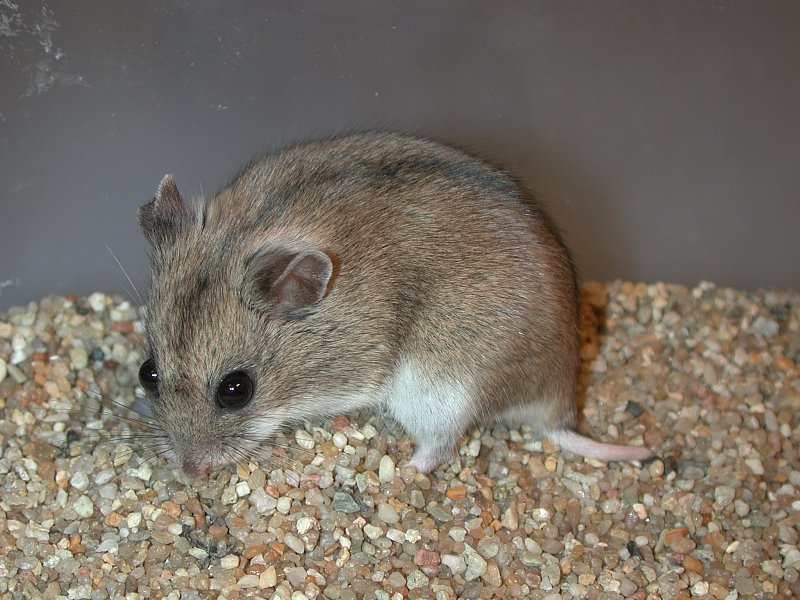
\includegraphics[width=0.7\linewidth]{curtatus.jpg}
\caption{Mongolian hamster (Allocricetulus curtatus) is a rodent species. Belongs to the family Cricetidae. Small, but larger than the mouse. The color is very light. The coat is flat. It is found in the south of Tuva, in China and in Mongolia.}\label{fig:curtatus}
\end{figure}

Experimental animals of the first study were two Mongolian hamsters (\textit{Allocricetulus curtatus}) with implanted epidural (located above the dura mater, the outer of the three shells covering the brain and spinal cord) EEG electrodes and intraperitoneal thermal and acceleration sensor. The animals were placed in a special chamber, the temperature of which decreased gradually by 1 degree per day for three weeks, from room temperature to 4 Celsius. At the same time, the duration of the illumination period was reduced gradually from 12 to 2 hours per day. The hamsters were provided with food \textit{ad libitum}, lighting and all necessary materials for the burrow. 

During this experiment, three physiological parameters of the animal were recorded: electroencephalographic (EEG) brain activity recorded from two electrodes; acceleration recorded from three accelerometers corresponding to three dimensions; and body temperature. Temperature measurement took place every 10 minutes. EEG and acceleration recording were performed at a frequency of 250 Hz. 

The recording of changes in body temperature continued throughout the experiment. EEG and accelerometer recordings were divided into 7 pieces with intervals of several hours. There was information about the start time of the recording in the data to the nearest second. For the analysis, we used only one EEG channel, since the second one recorded random noise and network crosstalk that did not correspond to physiological activity. Also, the records from only one accelerometer were used – the dynamics, not the direction, was of interest.






\subsection{The Naked Mole-rats Experiment}
\label{sec:Methods:The Naked Mole-rats Experiment}

\begin{figure}[H]
\centering
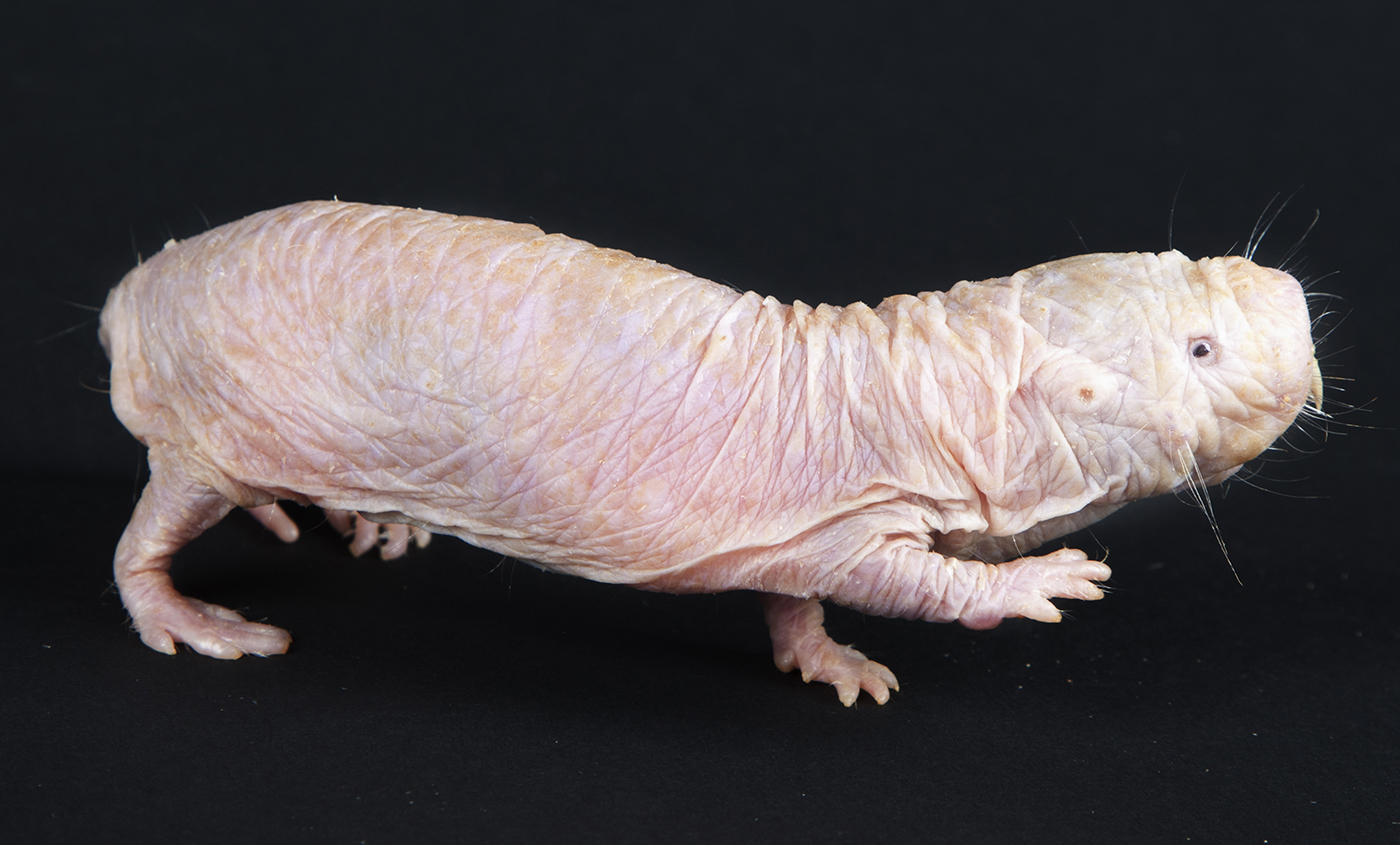
\includegraphics[width=0.7\linewidth]{nakedmolerat.jpg}
\caption{Naked mole-rat (\textit{Heterocephalus glaber}), or sand puppy, are burrowing rodents of the family Bathyergidae. The species is distinguished by unique features for mammals: a complex social organization of the colony, cold blood, insensitivity to some forms of pain. Appearance indicates the adaptation to the underground lifestyle. Found in East Africa, especially in Ethiopia.}\label{fig:nakedmolerat}
\end{figure}

Experimental animals of the second study were 4 naked mole-rats (\textit{Heterocephalus glaber}) with intraperitoneal thermal and acceleration sensor. The animals were placed in a special chamber, the temperature of which was constant. Day and night shifts were simulated in the chamber. The naked mole-rats were provided with food \textit{ad libitum}, lighting and all necessary materials for the burrow. 

During this experiment, two physiological parameters of the animal were recorded: acceleration recorded from three accelerometers corresponding to three dimensions; and body temperature. Temperature and acceleration measurement took place every 10 minutes.





\subsection{The Lactate Experiment}
\label{sec:Methods:The Lactate Experiment}

In the third experiment regular laboratory rat of the species \textit{Rattus norvegicus domestica} with EEG electrodes and intraperitoneal acceleration sensor were used. 33 rats were examined in the experiment. The rats were operated a week before the study. The holes were made in their heads, so that it would be possible to inject solutions into the ventricular system through them. 

Experimental animals were divided into two groups. The first group was infected with a solution of l-lactate on the first day. The second group was infected with d-lactate.  Both groups were administered a reference saline solution on the second day. 

During this experiment, two physiological parameters of the animal were recorded: EEG brain activity recorded from two electrodes; acceleration recorded from three accelerometers corresponding to three dimensions. EEG and acceleration recording were performed at a frequency of 250 Hz. 




\subsection{Lactate Receptors Phylogenetic Tree}
\label{sec:Methods:Lactate Receptors Phylogenetic Tree}

The amino acid sequences of the human HCA1, OR51E2 and GPR4 receptors were taken from the NCBI library \citep{Pruitt2007}. 

The BLAST program was used to search for homologous sequences \citep{Altschul1997}. Maximal target sequences for OR51E2 and GPR4 was 250 sequences; for HCA1 was 500 sequences. This was done to ensure that all chordates of all сlades are in the target search group. BLOSUM45 matrix was used to find distant relative genes. 

After all sequences were found, the Сlustalw software was used to build the multiple alignment and the corresponding phylogenetic tree with neighbor-joining method \citep{Thomopson1994,Saitou1987}. 

Finally, iTOL software was used for a convenient visualization of the phylogenetic tree \citep{Letunic2007}.











\newpage
\section{Results}
\label{sec:Results} 

\subsection{The Hamster Experiment}
\label{sec:Results:THe Hamster Experiment} 


\subsubsection{The Fist Hamster}
\label{sec:Results:The Hamster Experiment:The Fist Hamster} 

The first hamster began to hibernate at a temperature of 8 Celsius and demonstrated 8 bouts during 23 days. The hamster never woke up after the 8th bout, having failed to accumulate enough subcutaneous adipose tissue, which often happens in natural conditions.

\begin{figure}[H]
\centering
\begin{minipage}{.5\textwidth}
  \centering
  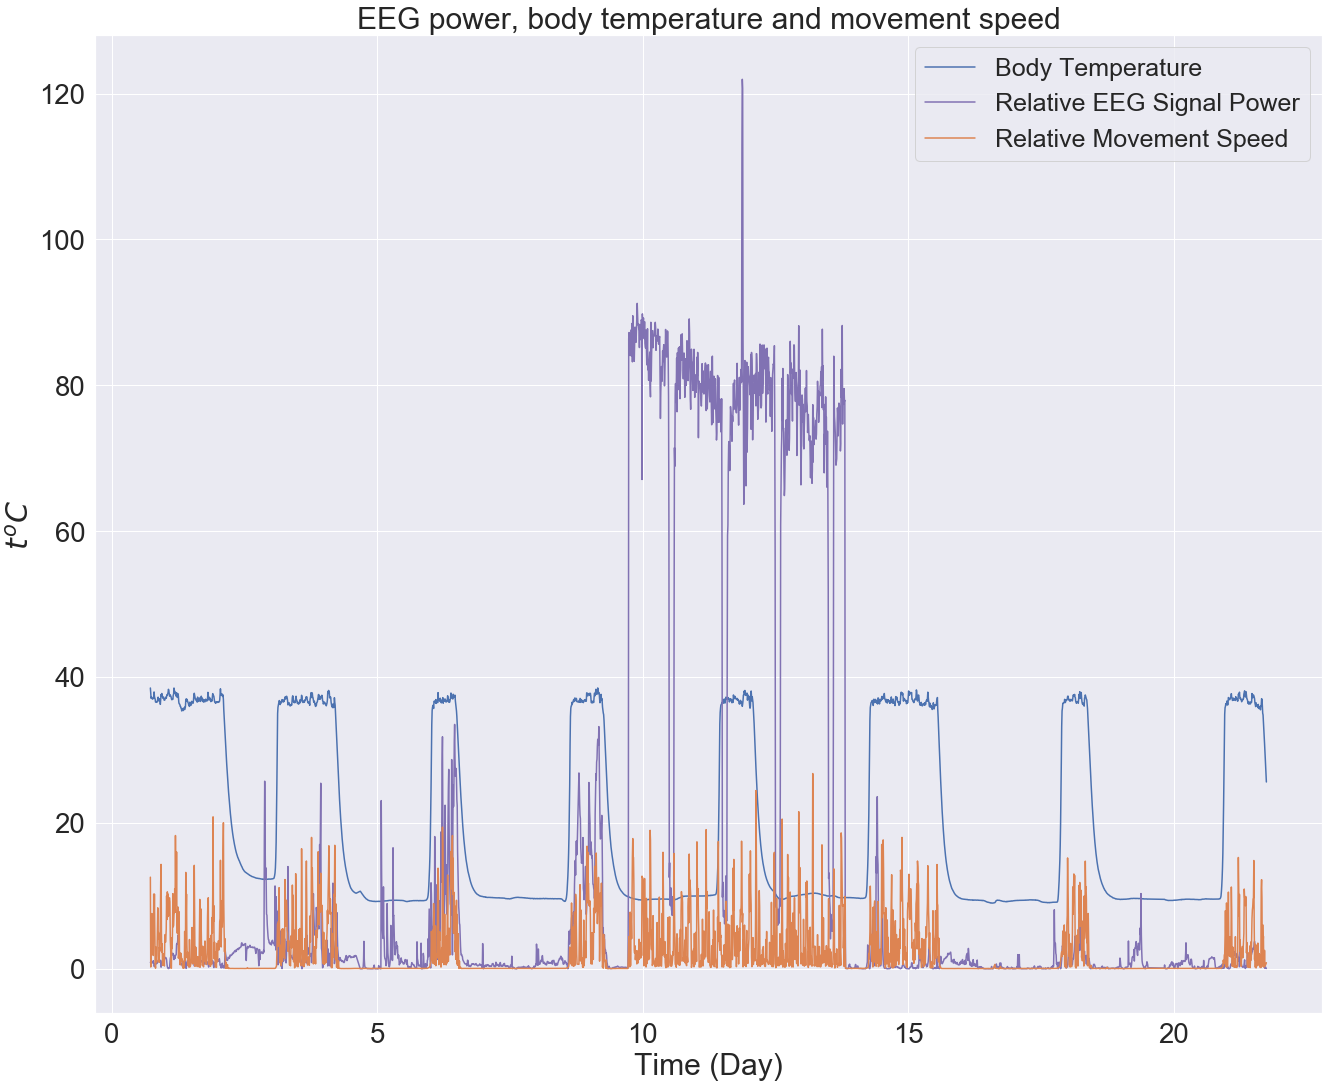
\includegraphics[width=\textwidth]{exp1_1.png}
  \captionof{figure}{The graph shows the body temperature of a hamster as a function of time, scaled movement speed and scaled values of EEG power. The part with a large artifact is not deleted. All measurements are presented.}\label{fig:exp1_1}
\end{minipage}%
\begin{minipage}{.5\textwidth}
  \centering
  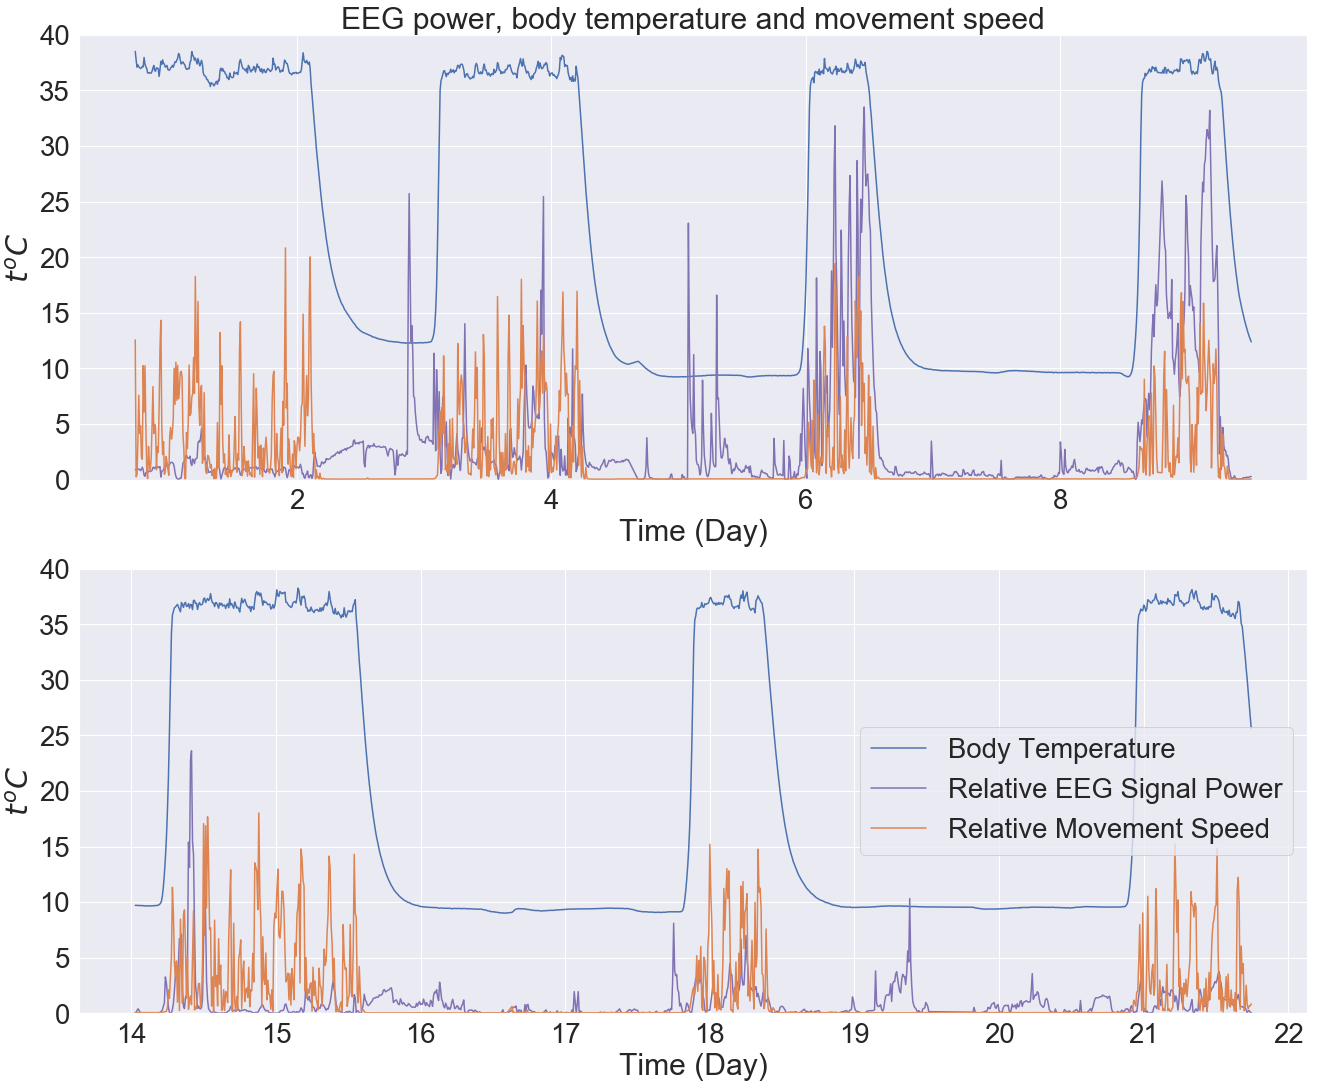
\includegraphics[width=\textwidth]{exp1_2.png}
  \captionof{figure}{The graph shows the body temperature of a hamster as a function of time, scaled movement speed and scaled values of EEG power. The part with a large artifact, located in the middle, is removed. The schedule is divided into two parts for convenience.}\label{fig:exp1_2}
\end{minipage}
\end{figure}

The first problem solved was matching the EEG, accelerometer and thermometer data in time. Therefore, the speed $ v_{x}(t_0, T) $ and the average EEG power of the signal $ P (t_0, T) $ were calculated over a time interval of 10 minutes for each of the seven EEG and accelerometer records. Also, the average power of a signal was obtained. The signal was previously filtered by a filter with a finite impulse response (FIR filter) in the frequency range 1–4 Hz denoted as $P(t_0, T)_{1-4Hz}$ and 4-8 Hz denoted as $ P(t_0, T)_{4-8Hz} $. 

\begin{figure}[H]
\centering
\begin{minipage}{.5\textwidth}
  \centering
  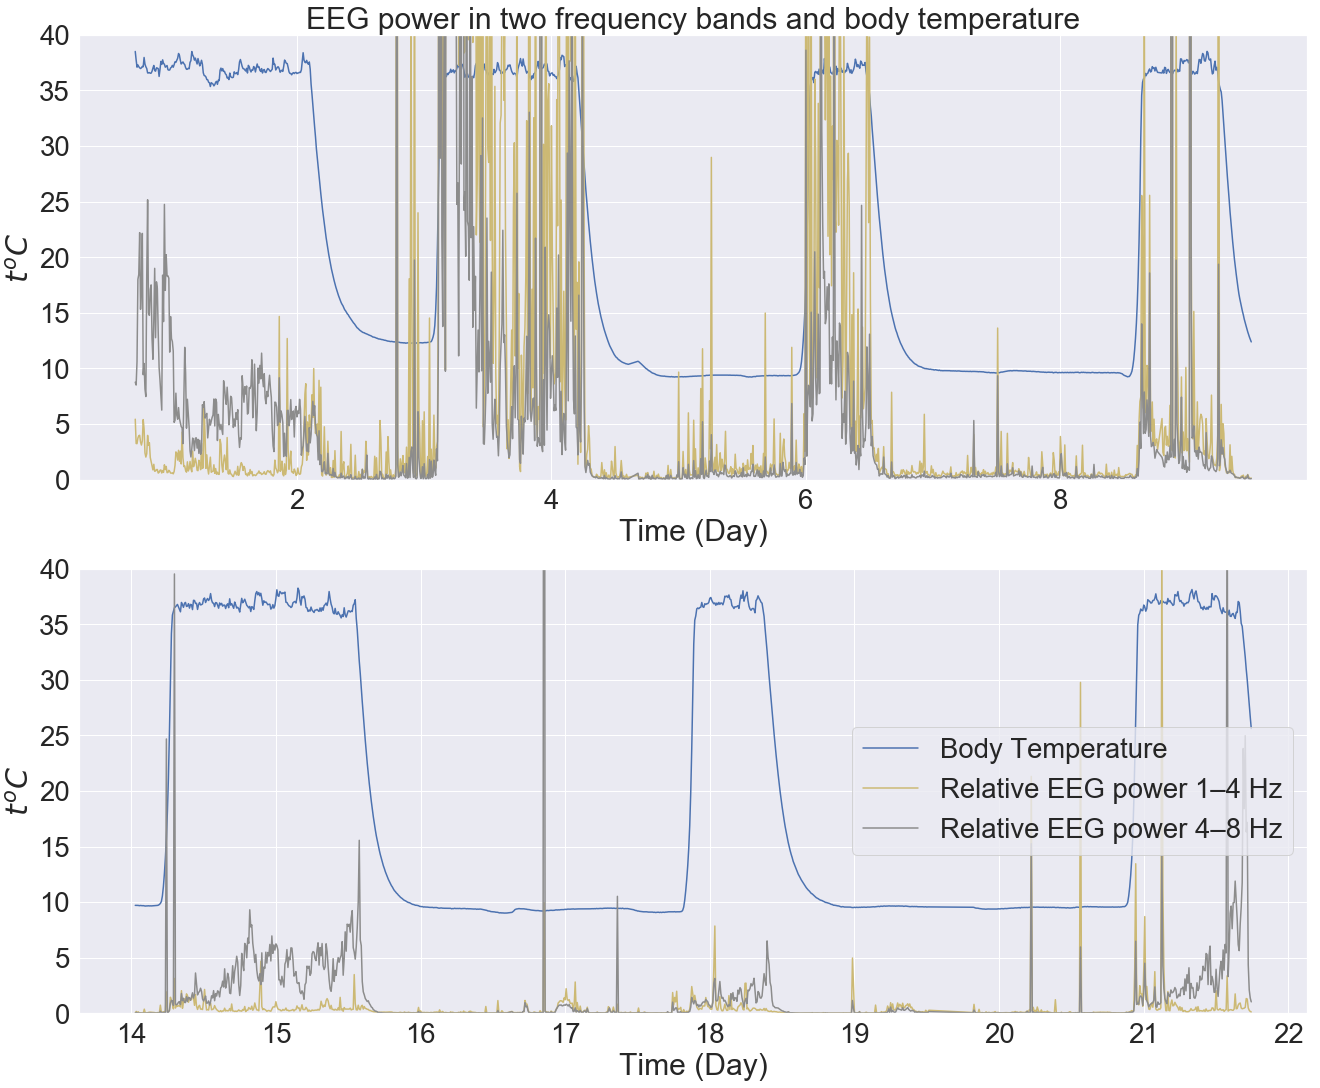
\includegraphics[width=\textwidth]{exp1_3.png}
  \captionof{figure}{The graph shows the hamster body temperature versus time and scaled EEG power values ​​in two different frequency bands (1-4 Hz and 4-8 Hz). The part with a large artifact, located in the middle of the record, is deleted. The graph is divided into two parts for convenience.}\label{fig:exp1_3}
\end{minipage}%
\begin{minipage}{.5\textwidth}
  \centering
  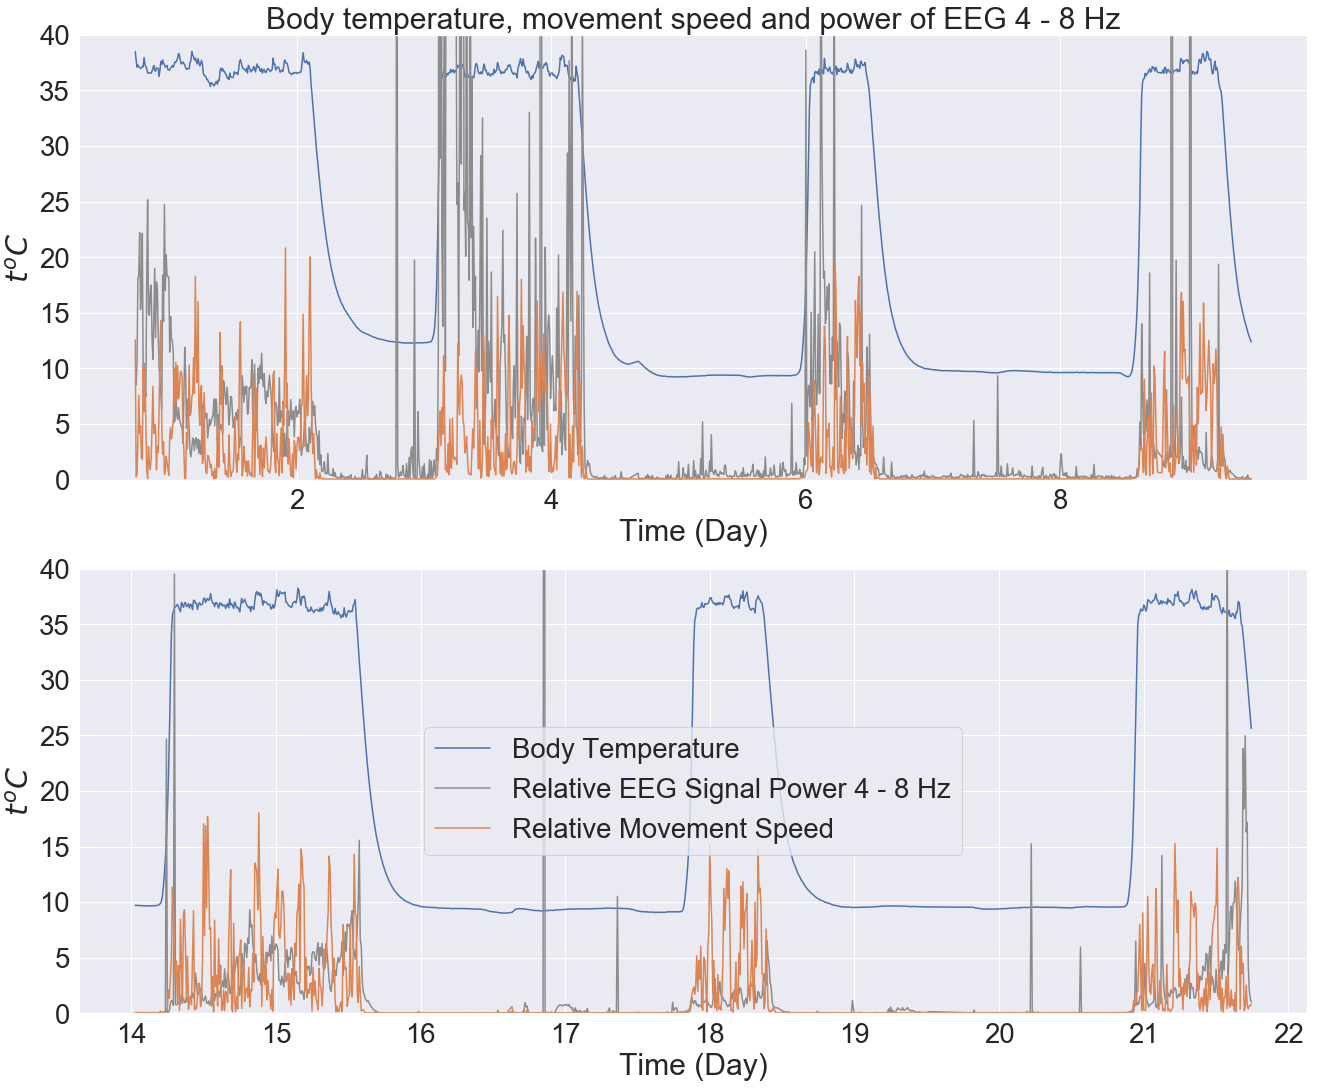
\includegraphics[width=\textwidth]{exp1_4.png}
  \captionof{figure}{The graph shows the body temperature of a hamster as a function of time, scaled movement speed and scaled values ​​of the EEG power in the frequency range 4--8 Hz. The part with a large artifact, located in the middle of the record, is deleted. The graph is divided into two parts for convenience.}\label{fig:exp1_4}
\end{minipage}
\end{figure}

The velocity over an interval of length $T$ can be calculated with the formula $ v_{x} (t_0, T) = \int_{t_0}^{t_0+T} | a_{x} (t) | dt $. In the case of physical signals, the average power over the same interval is calculated with the formula $ P (t_0, T) = \frac{1}{T}\int_{t_0}^{t_0+T}[x(t)]^2 dt $. The stable FIR filter was chosen for filtration, causing a smaller distorting of a signal with abrupt changes in amplitude. Artifacts caused by activity other than EEG may exceed the amplitude of the EEG for short periods of time and thus distort the result of other types of filters. As a result, vectors of 10-minute average speed and power values were obtained for each 10-minute time interval, which could be compared with the thermometer values. 

There is a high surge in EEG power and the speed of the animal that took place from 11 to 14 day. Such a signal is difficult to interpret. It must have been a lengthy artifact that was removed from the recording. 

\begin{figure}[H]
\centering
\begin{minipage}{.5\textwidth}
  \centering
  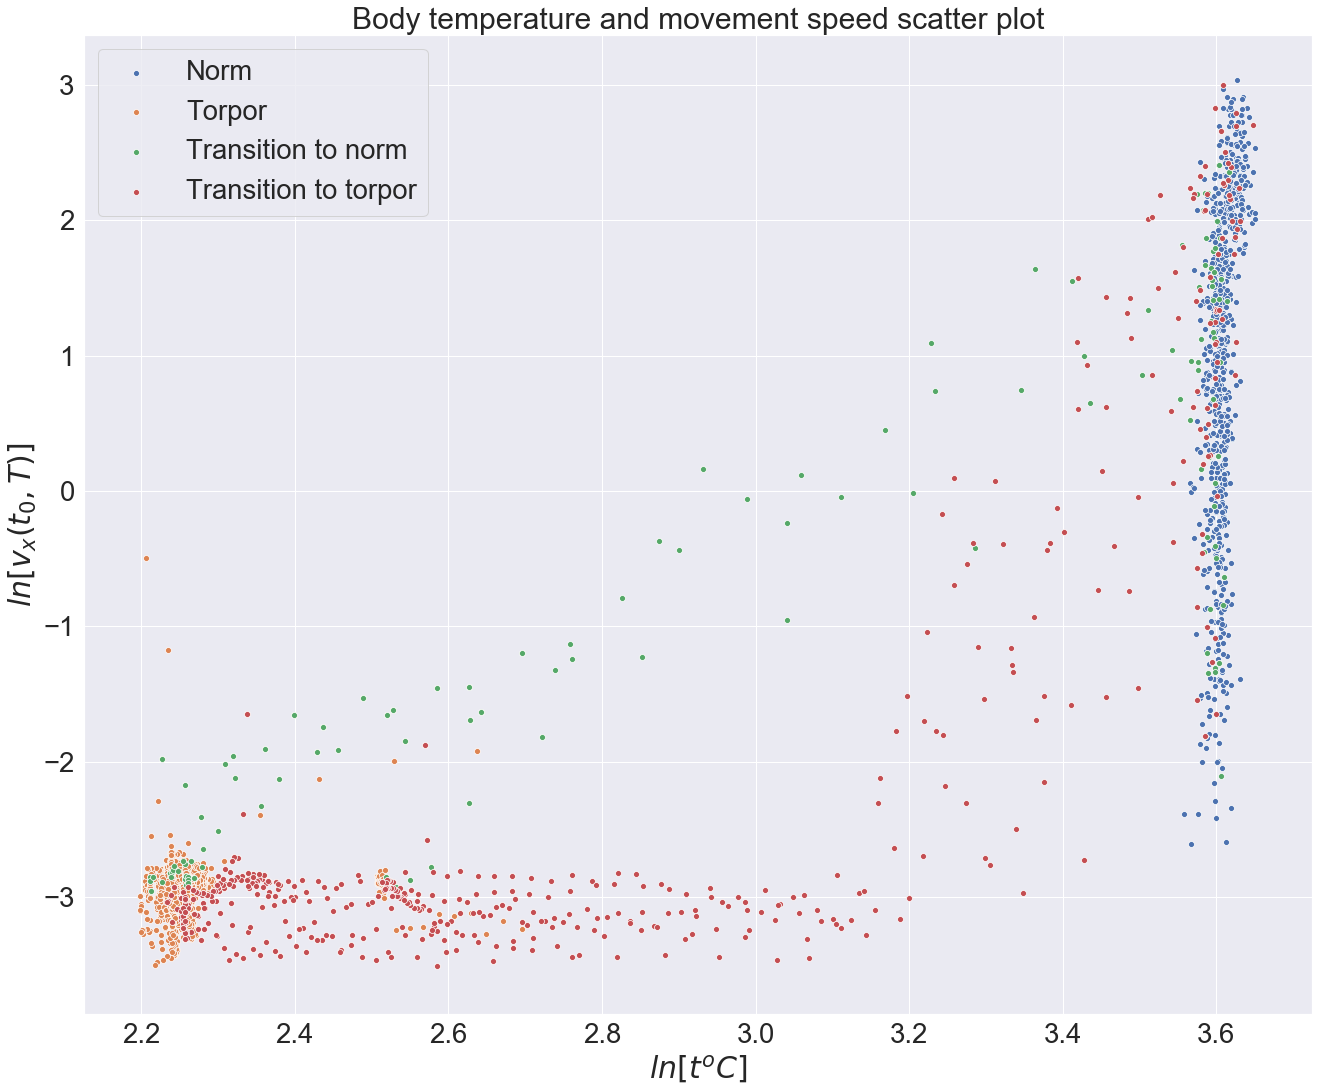
\includegraphics[width=\textwidth]{exp1_5.png}
  \captionof{figure}{The graph shows the scatterplot of the logarithm of the velocity of movement and the logarithm of body temperature, allowing to distinguish four states: norm, torpor, transition to torpor and transition to norm. States are highlighted in colors.}\label{fig:exp1_5}
\end{minipage}%
\begin{minipage}{.5\textwidth}
  \centering
  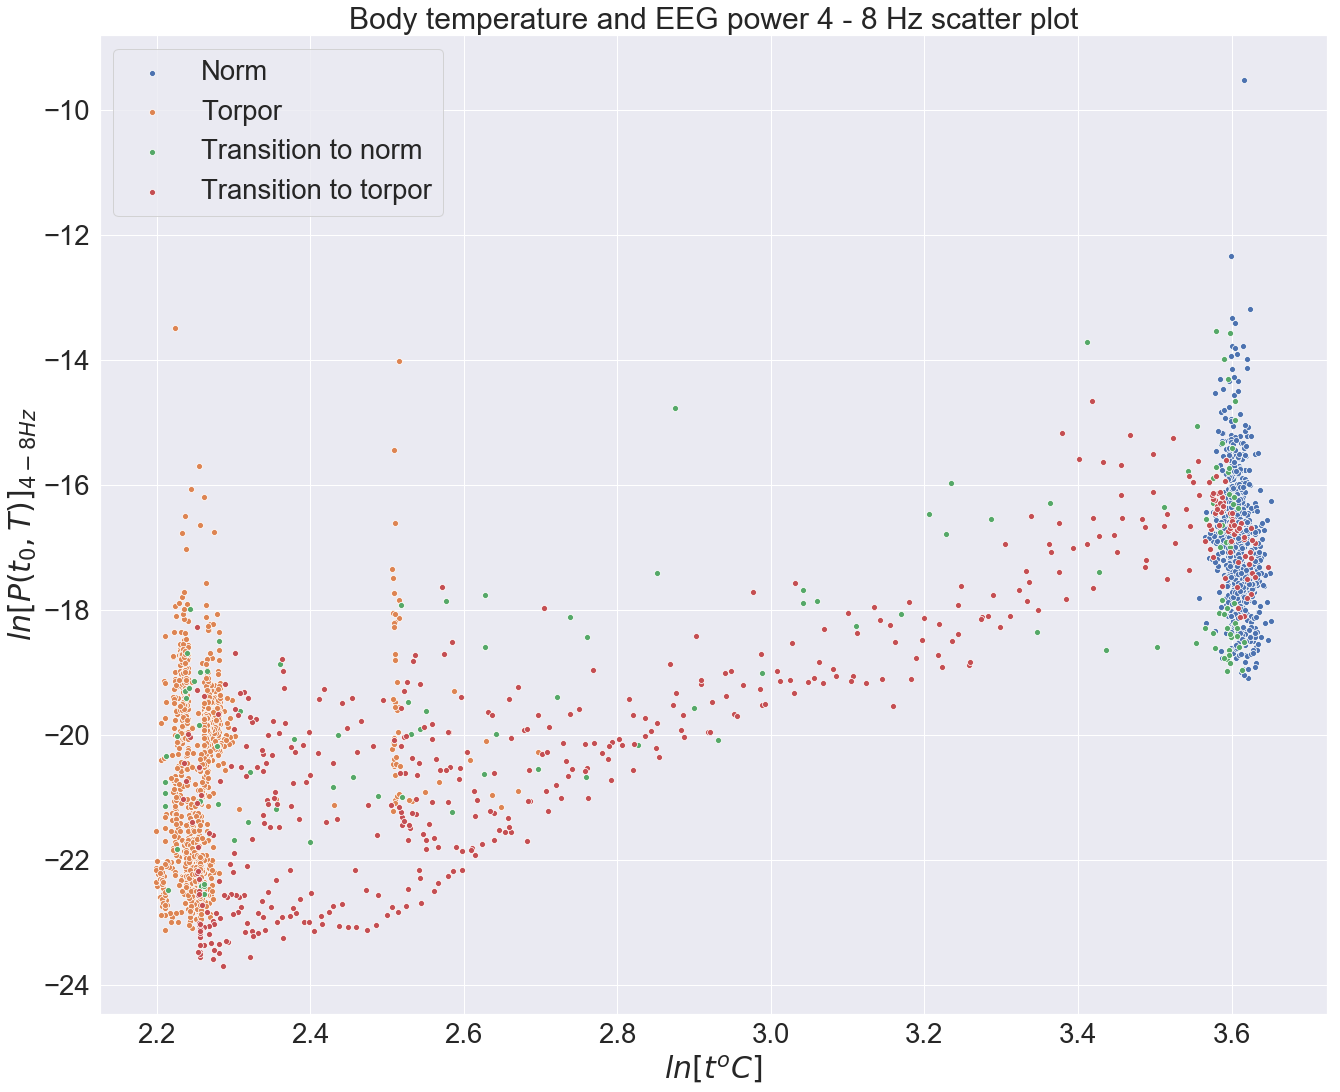
\includegraphics[width=\textwidth]{exp1_6.png}
  \captionof{figure}{The graph shows the scatterplot of the logarithm of body temperature and logarithm of the EEG power in the range of 4-8 Hz. 4 states are selected, corresponding to the diagram of the logarithm of the velocity of movement and the logarithm of temperature.}\label{fig:exp1_6}
\end{minipage}
\end{figure}

The scatterplots allow us to distinguish four states in which the hamster could have been: the normal state, the torpor state, the transition to torpor and the transition to the normal state. The scatterplot for the hamster’s body temperature and speed indicates that the speed was lower at low body temperatures. The hamster would fall into torpor and remain motionless in this case. At high temperatures the speed, on the contrary, was low. The hamster was awake often and moved more. During the transition from the normal state to torpor, it is clear that the hamster stopped and fell asleep, and then the body temperature began to drop. When switching from torpor to normal physiology, it is clear that the speed increased gradually, which means that the hamster was gradually warming up and was able to move more actively. 

The scatterplot for hamster body temperature and EEG power in the range from 4 to 8 Hz shows that the power was lower at low body temperatures. This can be explained by the energy-saving processes in the torpor state. Power, on the contrary, was greater at high temperatures. The hamster was awake and its brain used energy, which led to the electrical activity of the cells. However, in contrast to the speed, the power gradually increased when leaving the torpor state and decreased when entering this state. 

\begin{figure}[H]
\centering
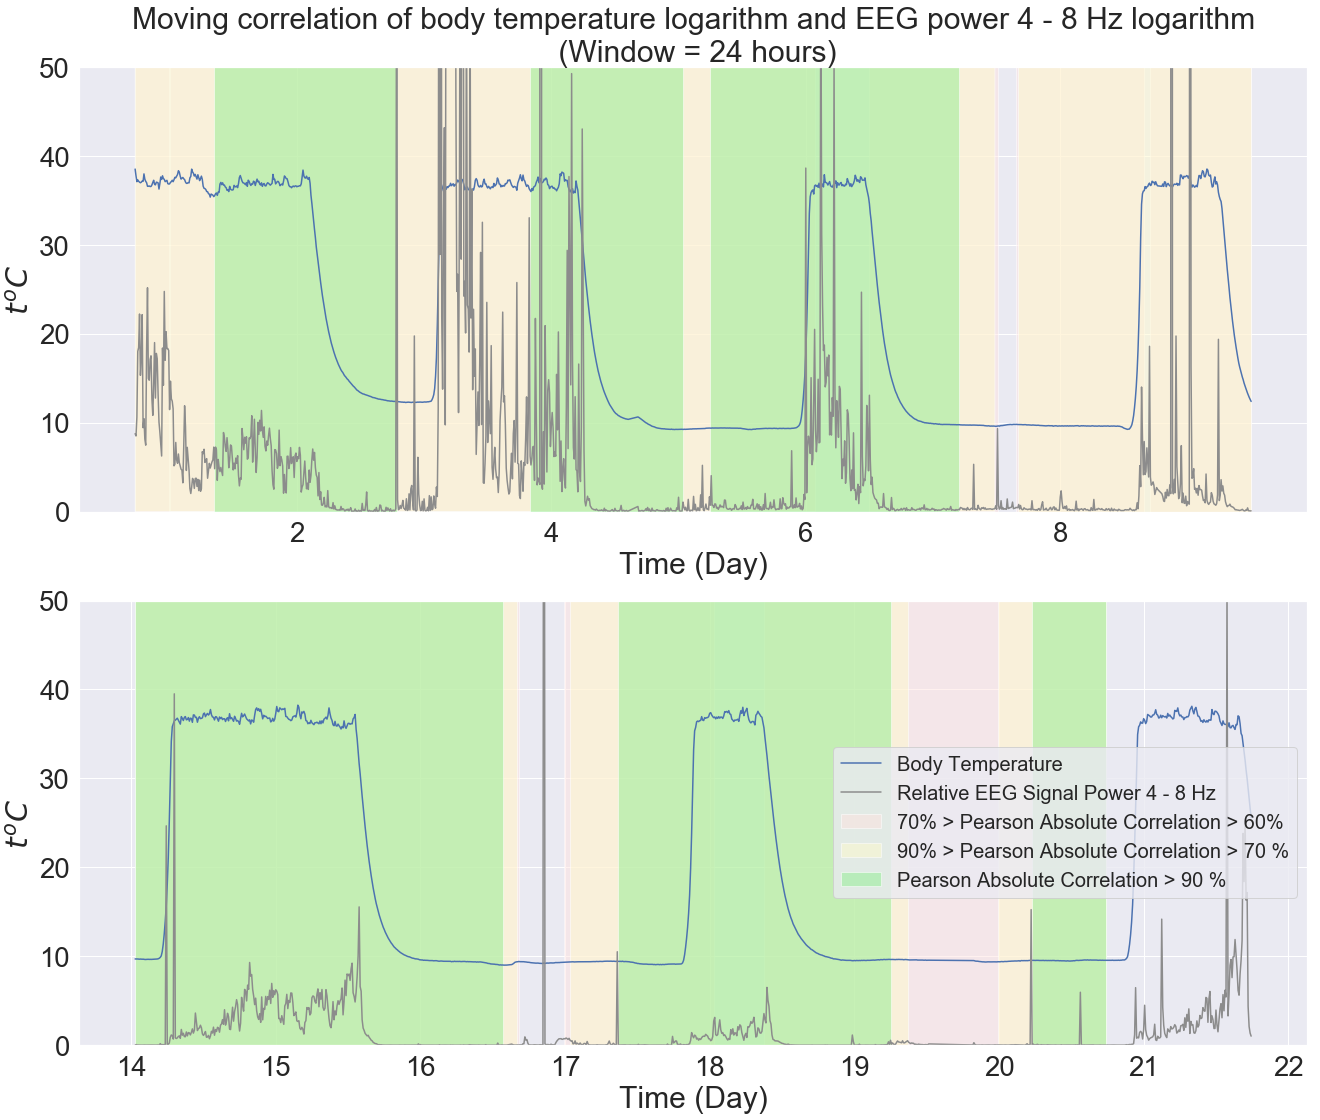
\includegraphics[width=0.7\linewidth]{exp1_7.png}
\caption{The graph shows the body temperature of the hamster as a function of time and scaled values of the EEG power in the range from 4 to 8 Hz. The part with a large artifact, located in the middle, is removed. The graph is divided into two parts for convenience. Red, yellow and green colors indicate areas where the Pearson correlation between the logarithm of hamster's body temperature and logarithm of EEG power values are significant and have a high value. }\label{fig:exp1_7}
\end{figure}

The sliding window method for Pearson correlation made it possible to establish the presence of a significant correlation of power and body temperature at different time intervals of the experiment. Areas with significant Pearson correlation between the logarithm of hamster's body temperature and the logarithm of EEG power values were depicted as time series. Сorrelation significance was indicated by color (red, yellow and green). We can witness that the highest correlation between the signals was observed during the transition from state to state. 

\subsubsection{The Second Hamster}
\label{sec:Results:The Hamster Experiment:The Second Hamster} 

\begin{figure}[H]
\centering
\begin{minipage}{.5\textwidth}
  \centering
  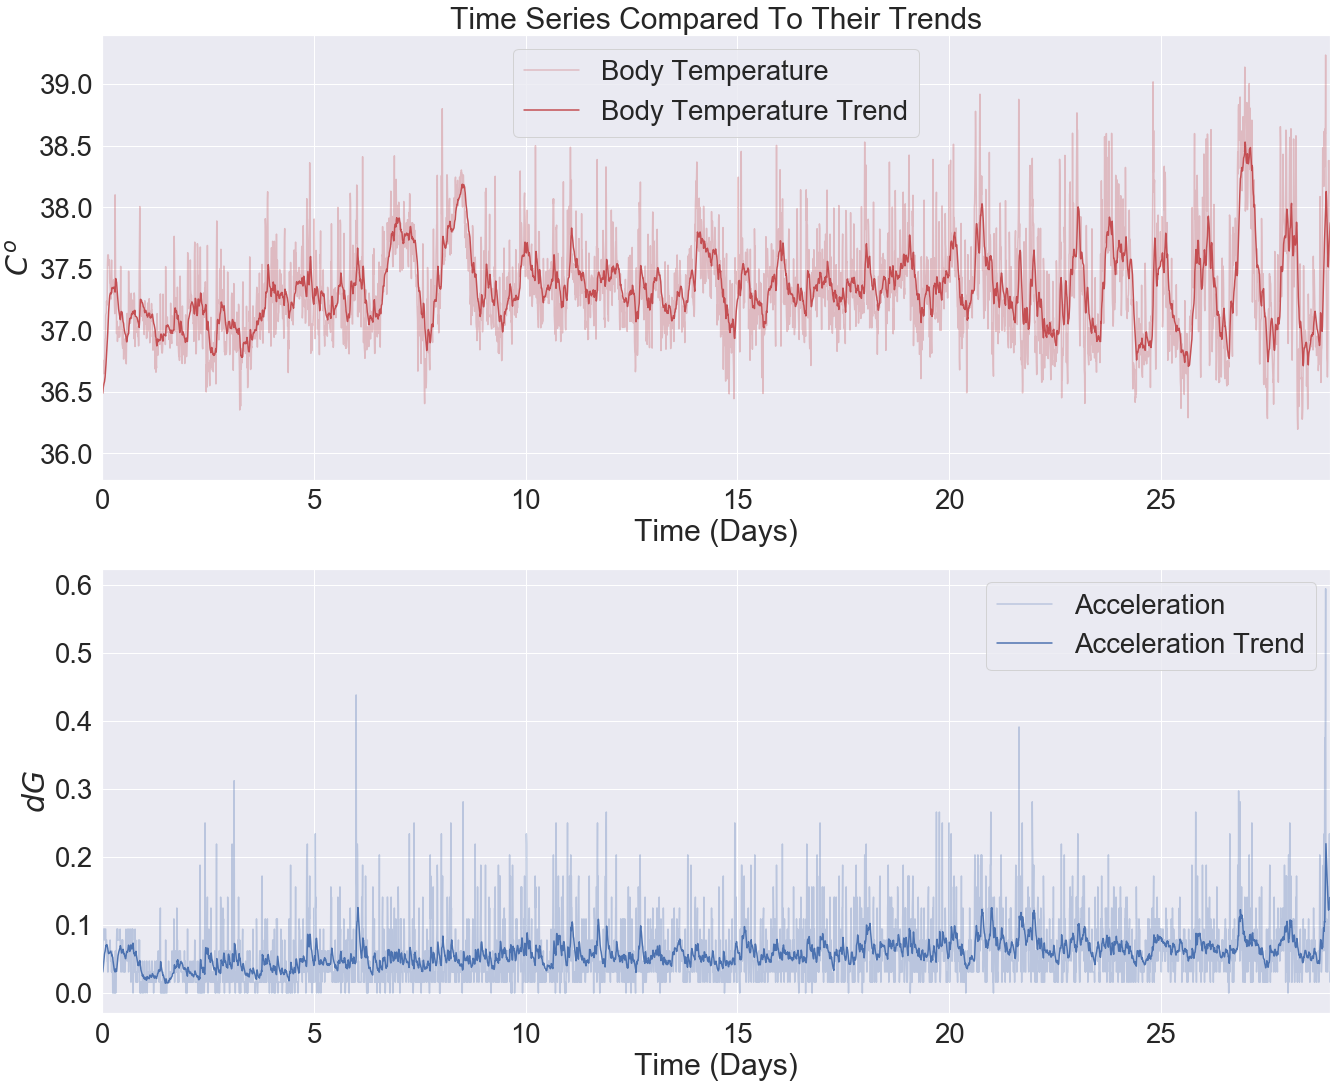
\includegraphics[width=\textwidth]{exp2_1.png}
  \captionof{figure}{Trends of body temperature and acceleration of a hamster against the background of time series}\label{fig:exp2_1}
\end{minipage}%
\begin{minipage}{.5\textwidth}
  \centering
  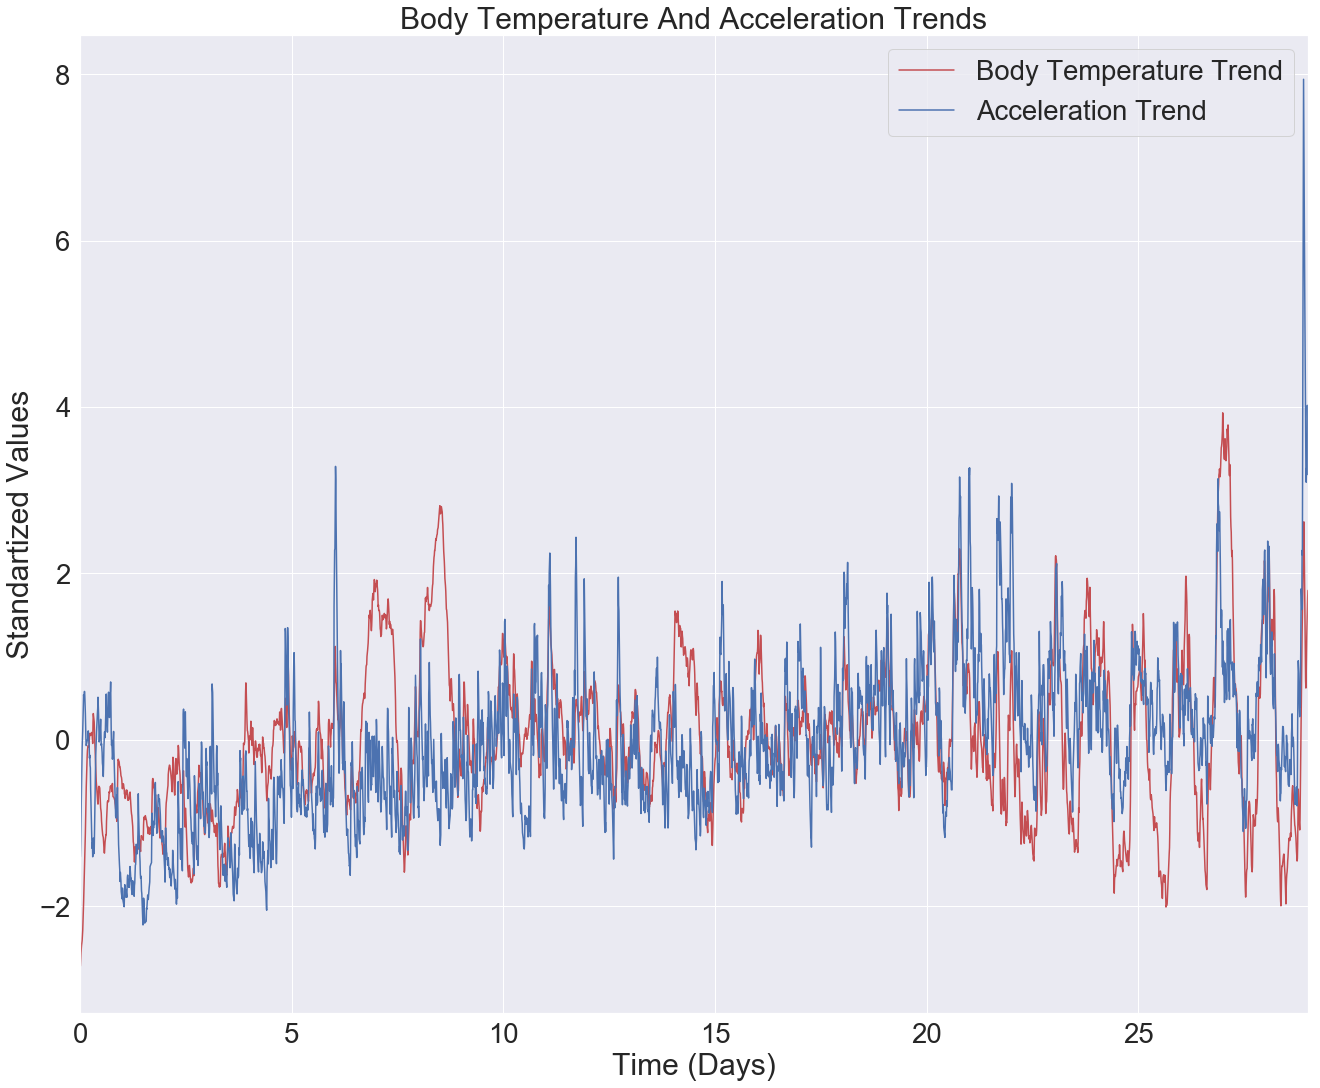
\includegraphics[width=\textwidth]{exp2_2.png}
  \captionof{figure}{Trends of body temperature and hamster acceleration superimposed.}\label{fig:exp2_2}
\end{minipage}
\end{figure}

The second hamster did not hibernate at all, but demonstrated a different strategy for survival in such conditions. Unlike the first hamster, the second managed to survive. 

First, a trend was identified for accelerometer and temperature data. This was done using simple exponential smoothing with smoothing factor equal to $0.1$. Smoothing factor is denoted as $\alpha$. Exponential smoothing is given by the formulas: $s_0 = x_0; s_t = \alpha x_t + (1 - \alpha) s_{t-1}, t > 0$. Unlike the first case, not the average speed was used, but the acceleration power at 10-minute time intervals. The formula by which power is calculated is given in the previous section.

Then two trends were superimposed on each other. It can be seen with the naked eye that there is a relationship between the two trends, especially at the end of the record. To test this, the same approach was used as with the first hamster.

\begin{figure}[H]
\centering
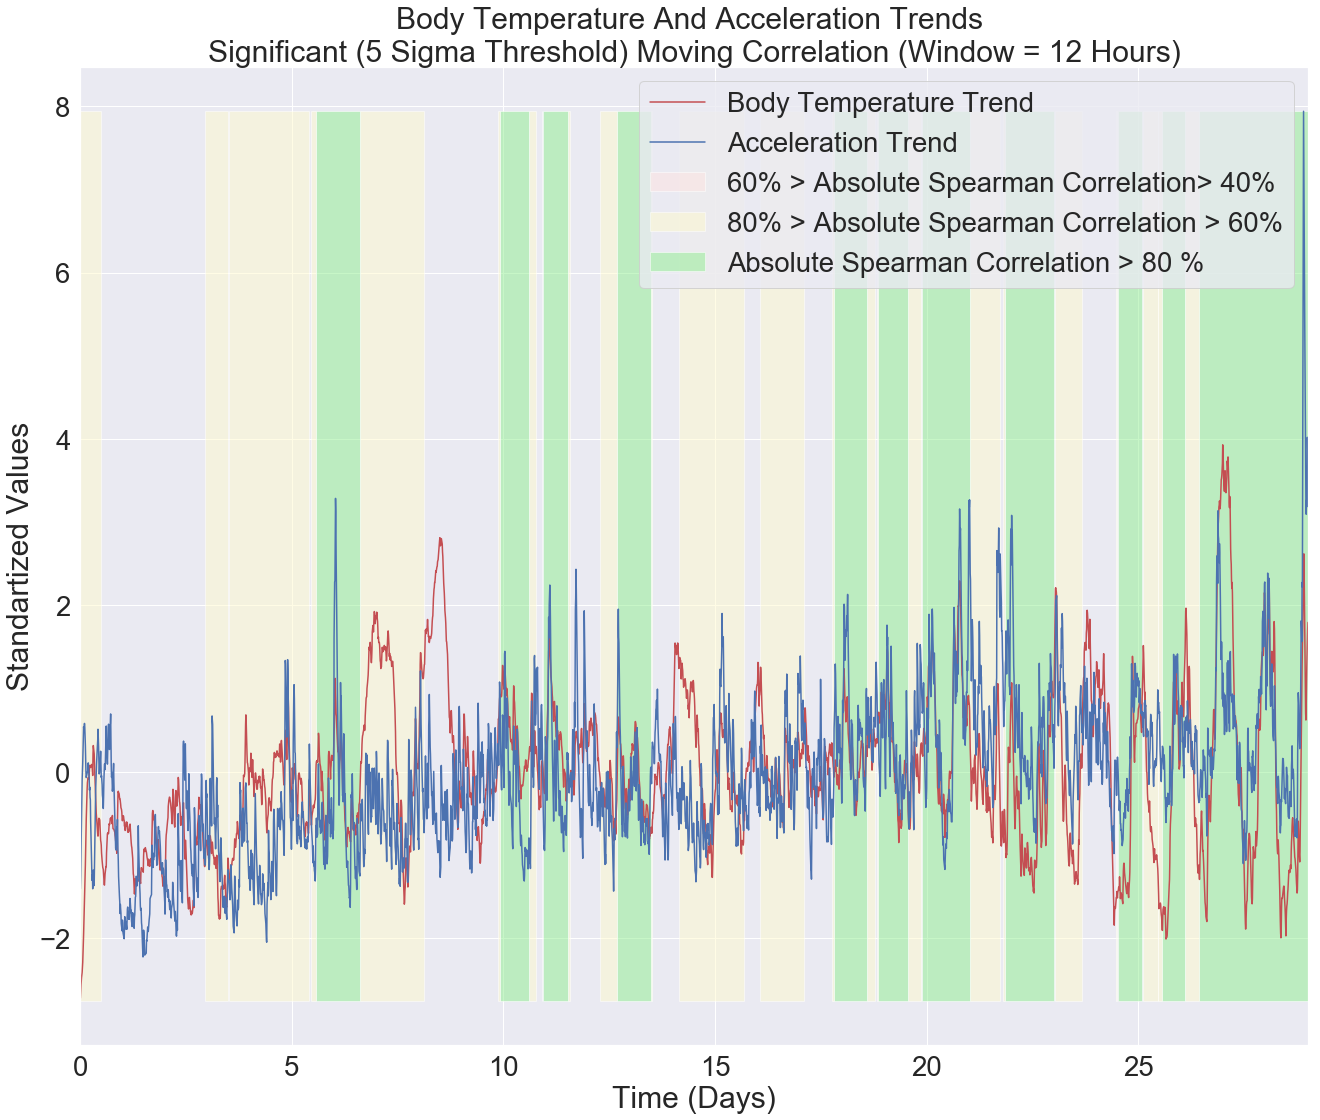
\includegraphics[width=0.7\linewidth]{exp2_3.png}
\caption{The graph shows the body temperature of the hamster as a function of time and scaled values of the speed. Red, yellow and green colors indicate areas where the Sperman correlation between the hamster's body temperature and speed values are significant and have a high value.}\label{fig:exp2_3}
\end{figure}

The sliding window method for Spearman correlation made it possible to establish the presence of a significant correlation of power and body temperature at different time intervals of the experiment. Areas with significant Pearson correlation between the hamster's body temperature and the EEG power values were depicted as time series. Сorrelation significance was indicated by color (red, yellow and green). We can observe that there is a strong correlation at the end of the experiment. 

\subsection{The Naked Mole-rats Experiment}
\label{sec:Results:The Naked Mole-rats Experiment}

\begin{figure}
  \centering
  \begin{subfigure}[b]{0.4\linewidth}
    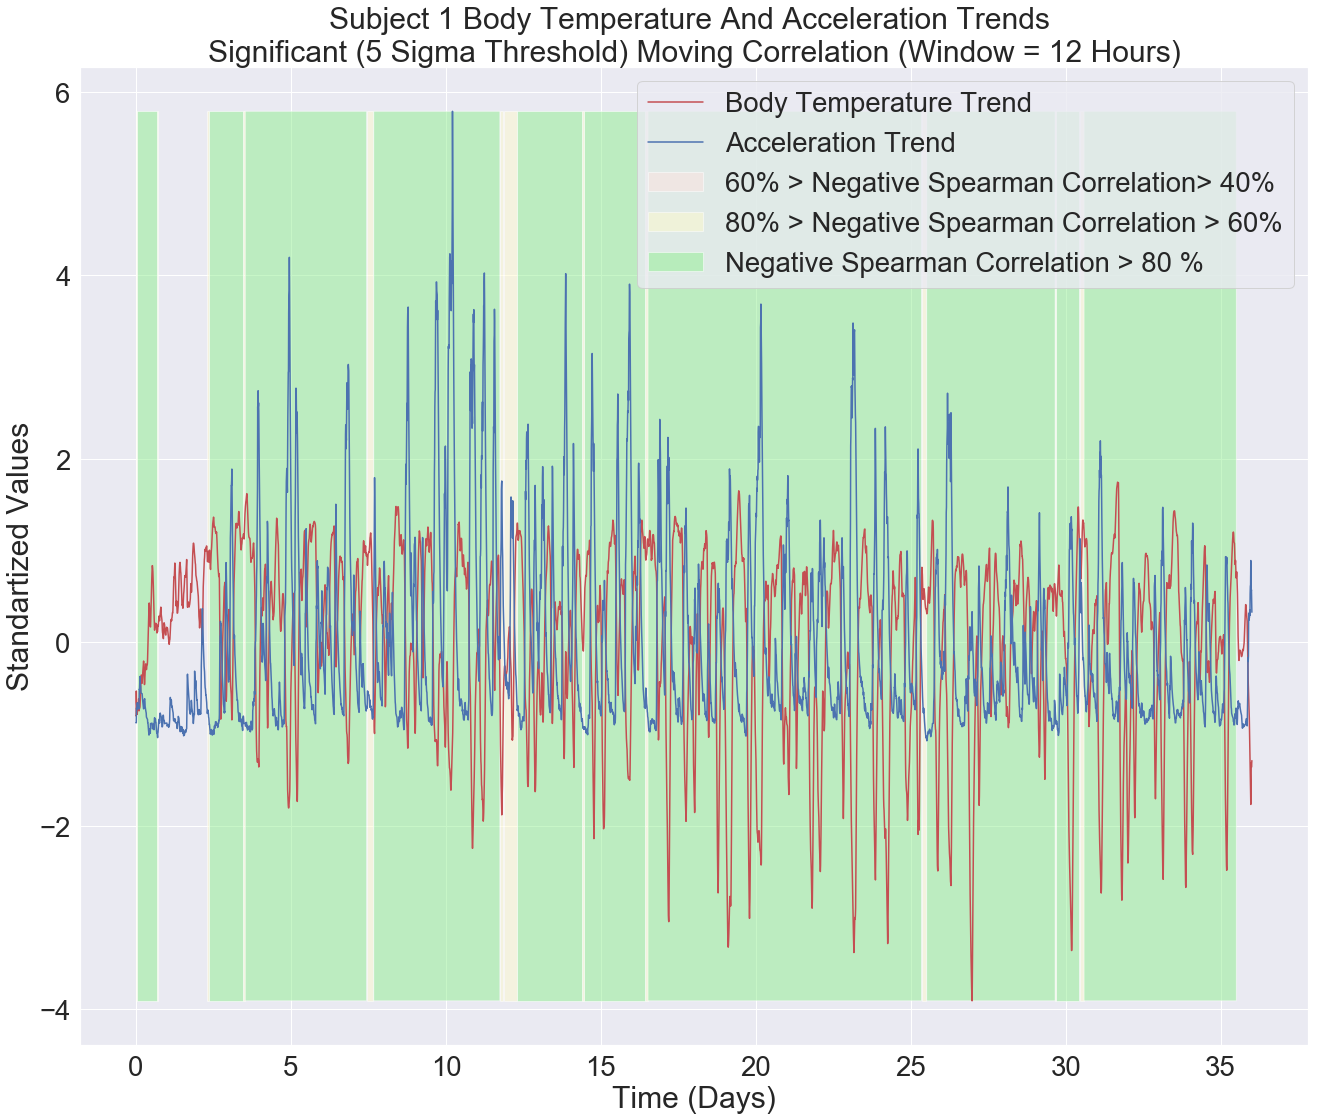
\includegraphics[width=\linewidth]{exp3_1.png}
     \caption{Subject 1}
  \end{subfigure}
  \begin{subfigure}[b]{0.4\linewidth}
    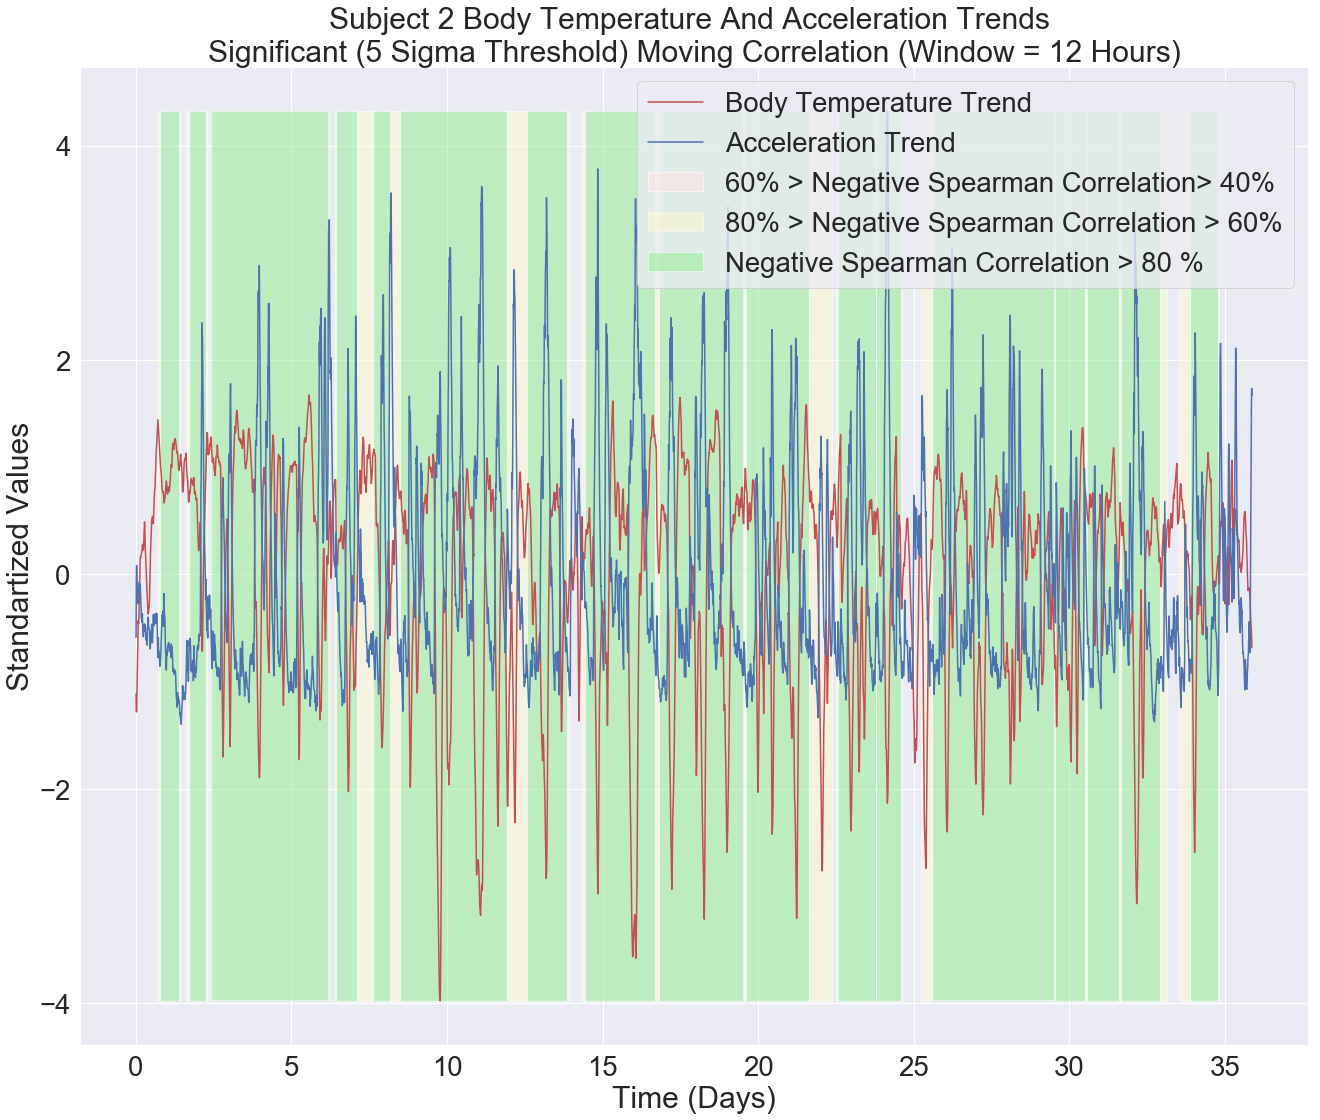
\includegraphics[width=\linewidth]{exp3_2.png}
    \caption{Subject 2}
  \end{subfigure}
  \begin{subfigure}[b]{0.4\linewidth}
    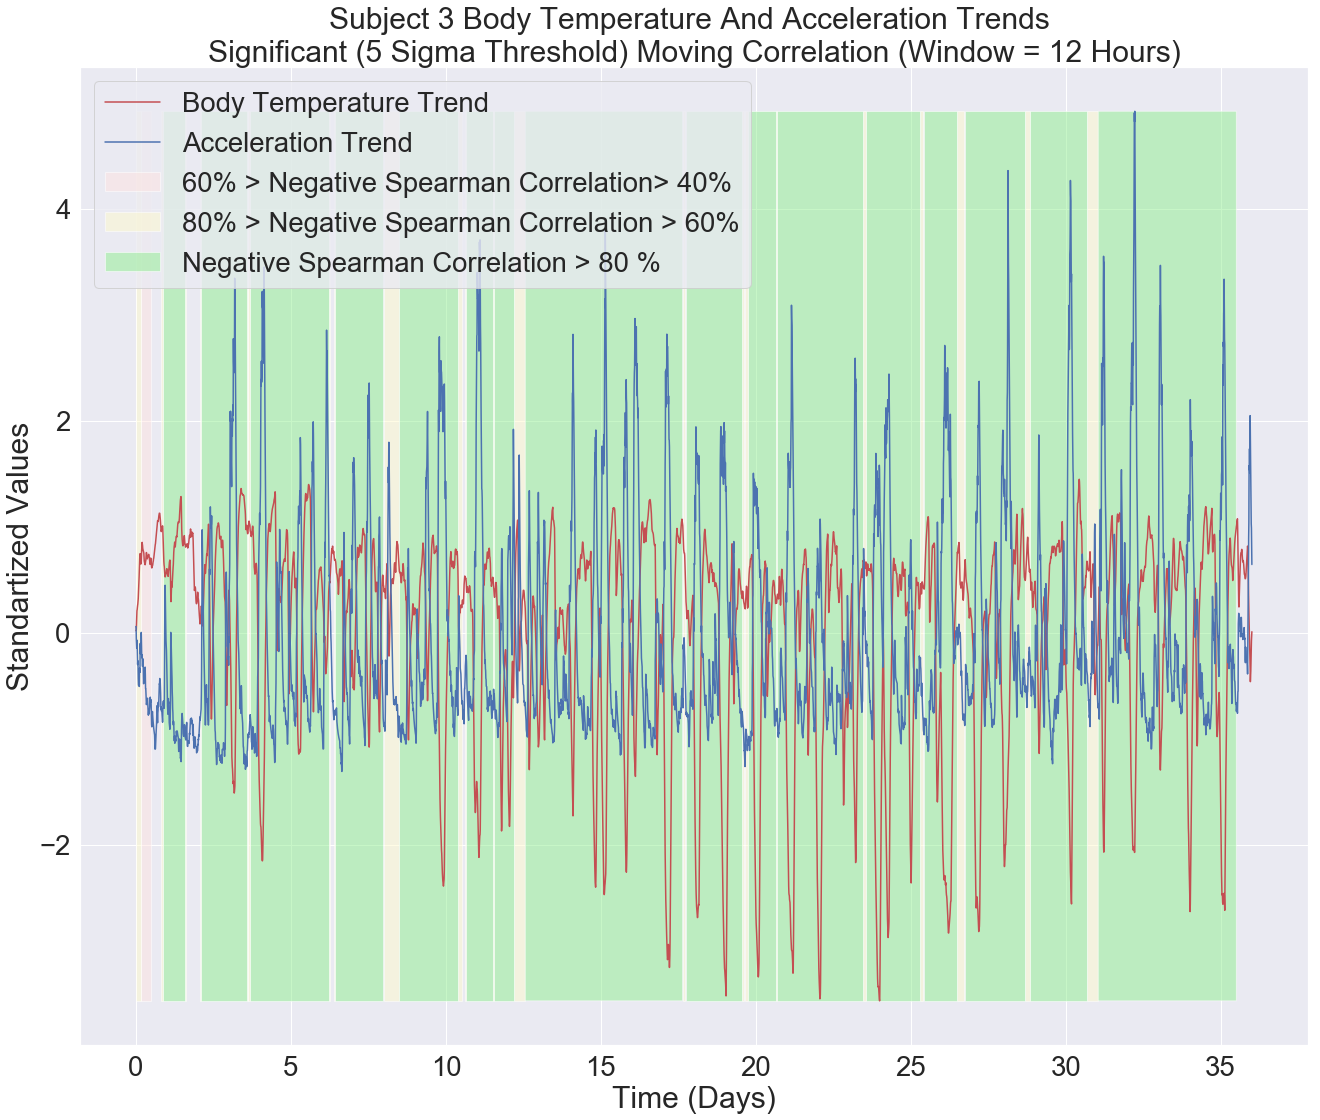
\includegraphics[width=\linewidth]{exp3_3.png}
    \caption{Subject 3}
  \end{subfigure}
  \begin{subfigure}[b]{0.4\linewidth}
    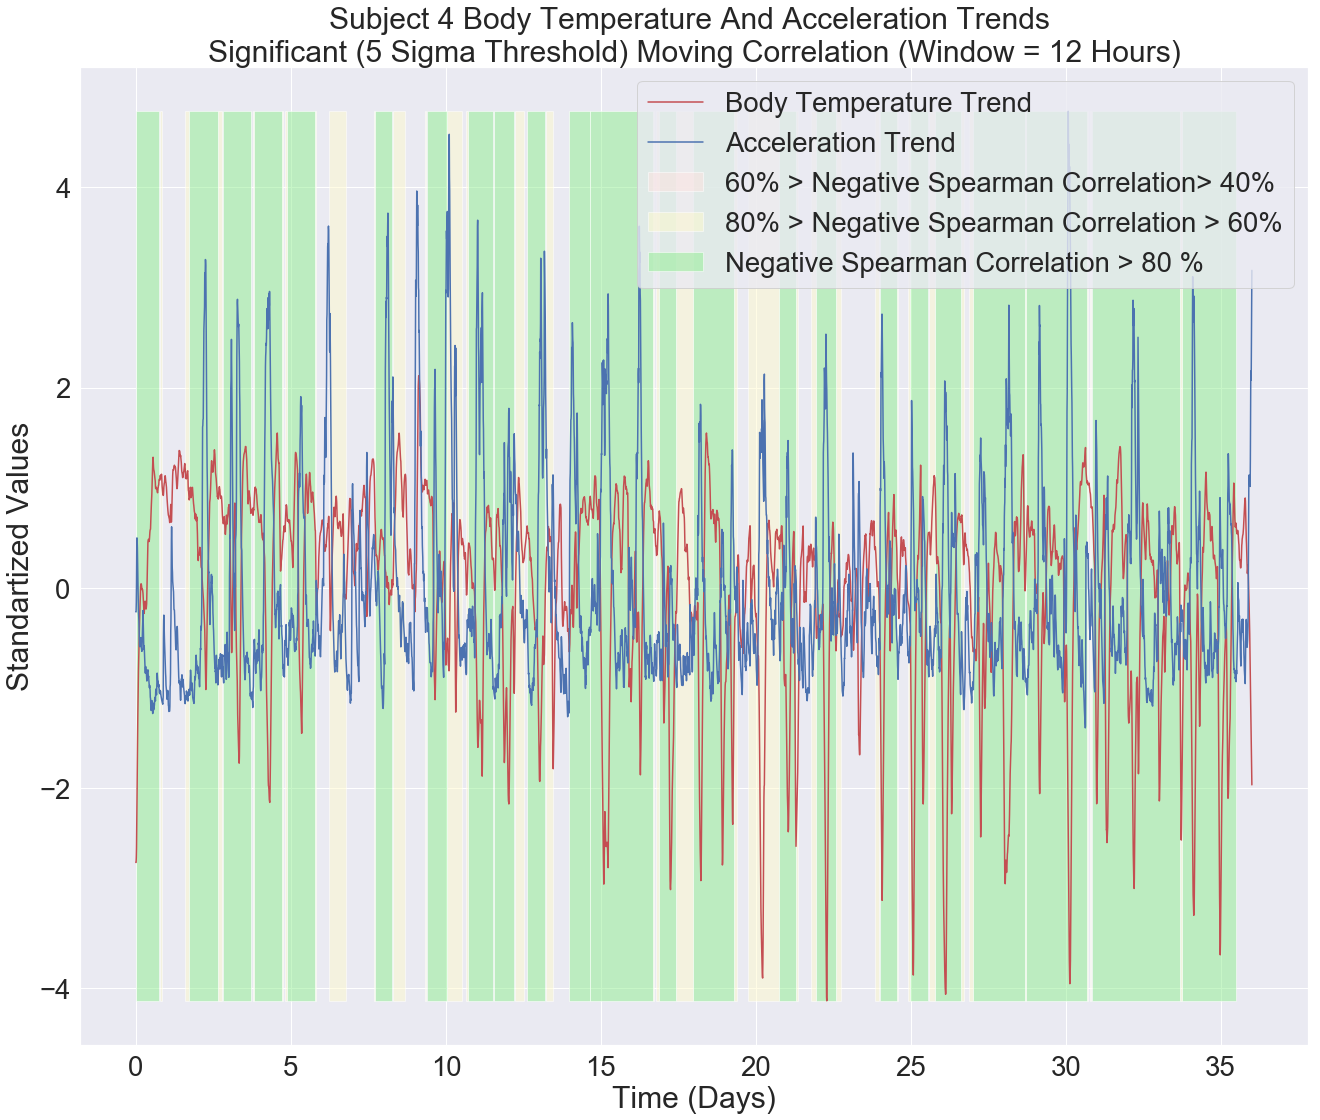
\includegraphics[width=\linewidth]{exp3_4.png}
    \caption{Subject 4}
  \end{subfigure}
  \caption{The picture shows a moving negative correlation of average acceleration and body temperature of 4 naked mole-rats at 10 minute time intervals. The graphs show that when an animal increases its speed, its body temperature drops. The x axis is time. The y axis is the standardized trends values of time series. Different colors of the background indicate a sliding correlation, highlighting the parts of the graph in the case of a larger effect for this window.
}
  \label{fig:exp3}
\end{figure}

The same approach as in the previous experiment was used to analyze the time series obtained for naked mole-rats. The only exception was that it was not necessary to isolate the trend.
It can be seen that the trend can be traced very well without pre-processing, but the correlation between trends is rather negative than positive. Therefore, the same Spierman correlation was used, but negative correlation values were considered.

The sliding window method for Spearman correlation made it possible to establish the presence of a significant correlation of power and body temperature at different time intervals of the experiment for naked mole-rats. Areas with significant Pearson correlation between the hamster's body temperature and the EEG power values were depicted as time series. Сorrelation significance was indicated by color (red, yellow and green). We can observe that there is a strong correlation at the end of the experiment. 



\subsection{The Lactate Experiment}
\label{sec:Results:The Lactate Experiment}

\begin{figure}[H]
\centering
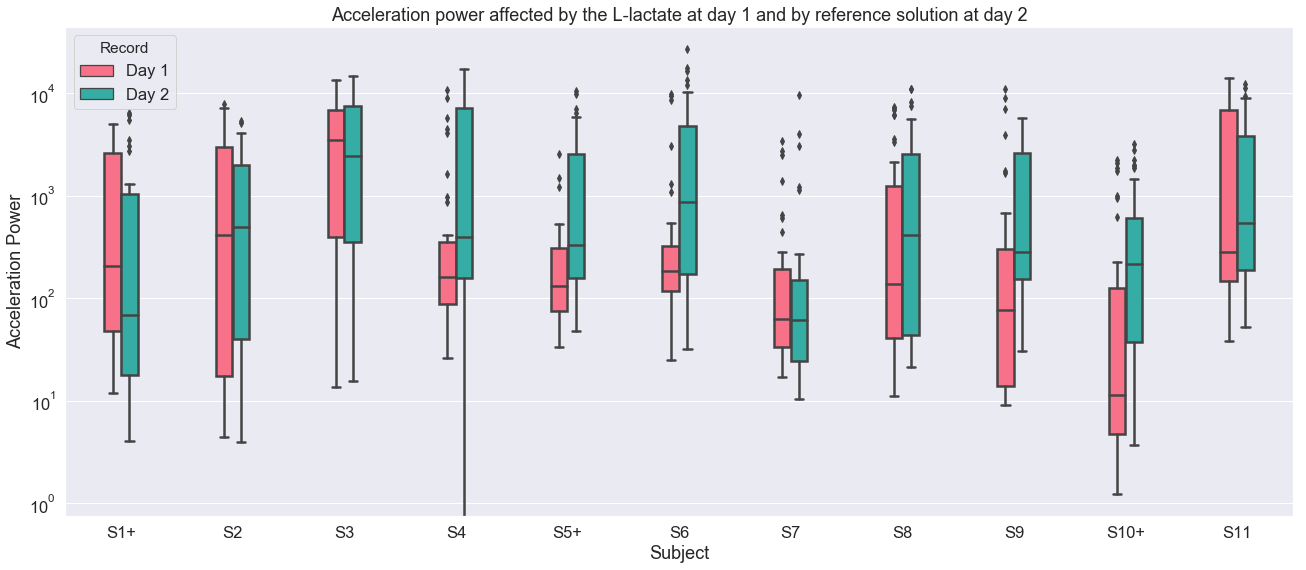
\includegraphics[width=\linewidth]{exp4_1.png}
\caption{The picture shows 22 boxplot items. Each pair refers to one experimental animal. The boxplot items corresponding to the first experimental day are pink, and the ones corresponding to the second are green. On the x-axis, the code names of experimental animals are plotted. The y-axis represents the distribution of the acceleration powers over 10 minute time intervals. On the first day l-lactate was administered to the animal. On the second day reference solution was administered to the animal. A plus in the animal code name denotes a significant (p < 0.05) with Bonferroni correction difference between distributions on the first and second day.
}\label{fig:exp4_1}
\end{figure}

At first, the recording of the acceleration of each subject was divided into 10 minute intervals. The signal power was calculated at each such interval. Thus, the power distribution was obtained at five-minute intervals. Only the first six hours of recording were taken into account, because the effect of lactate was expected to be observed throughout them. After six hours, lactate is usually metabolized. 

For each subject, the Wilcoxon test for the power distribution for the first and second days was calculated. Thereafter, the Bonferroni correction was made. For those subjects for whom it turned out to establish a significant difference between the distribution of power for two different days, a contingency matrix was constructed. The columns of the conjugacy matrix were enantiomers of lactate, and the rows were the days when less activity was observed.

Contingency matrix was used to test the hypothesis of a relationship between two features (enantiomers of lactate, less activity day). For this purpose the Fisher's exact test was calculated. The test did not show any significant difference (prior odds ratio $= 0.5$, $p-value = 1.0$). 


\begin{figure}[H]
\centering
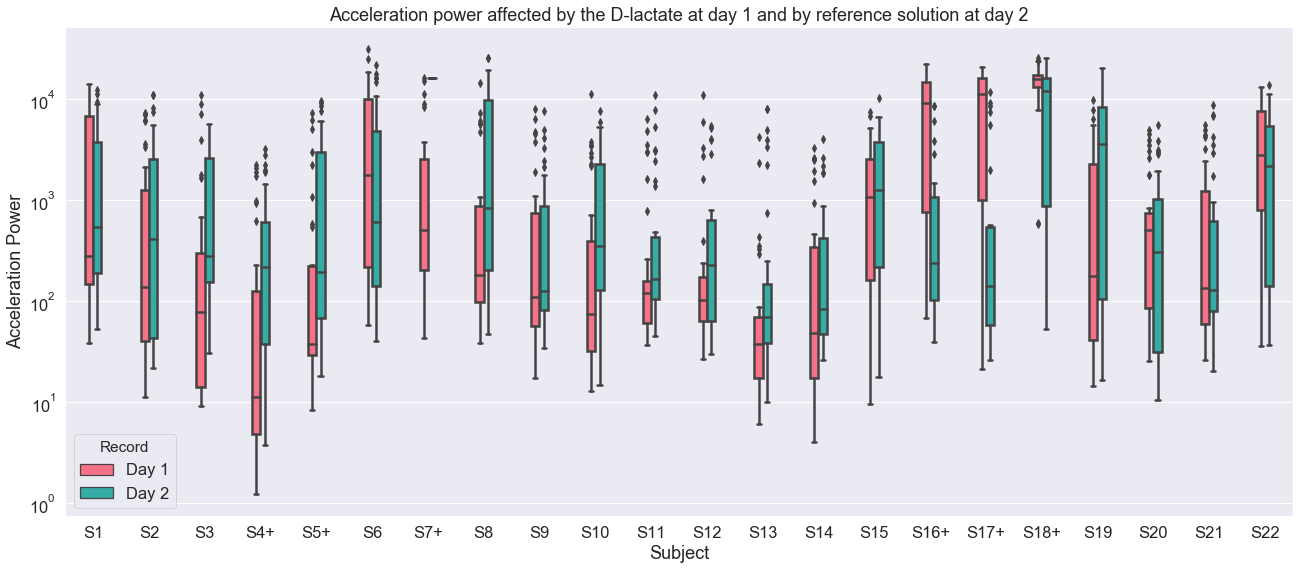
\includegraphics[width=\linewidth]{exp4_2.png}
\caption{
  The picture shows 44 boxplot items. Each pair refers to one experimental animal. The boxplot items corresponding to the first experimental day are pink, and the ones corresponding to the second are green. On the x-axis, the code names of experimental animals are plotted. The y-axis represents the distribution of the acceleration powers over 10 minute time intervals. On the first day d-lactate was administered to the animal. On the second day reference solution was administered to the animal. A plus in the animal code name denotes a significant (p < 0.05) with Bonferroni correction difference between distributions on the first and second day.
}\label{fig:exp4_2}
\end{figure}

\subsection{Lactate Receptors Phylogenetic Tree}
\label{sec:Results:Lactate Receptors Phylogenetic Tree}

Since the tree is large (750 sequences), it is not possible to put it in this report. A detailed image of the tree can be found in the appendix to the report. Following the link you can find three different trees: linear, circle, unrooted. The length of the branches and the number of clades is the same for each of the trees.

The resulting tree can be divided into three main branches corresponding to the target receptors (purple – HCA1; green - OR51E2; red - GPR4). Orthologs of the HCA1 protein among mammals belong to the HCA1 branche. OR51E2 proteins orthologs are found in all vertebrats except fish and amphibians. GPR4 proteins orthologs are found in all vertebrates in general. 

For the HCA1 protein, the closest branch of homologous proteins (hydroxycarboxylic acid receptor 2-like and 3-like) present in mammals and in other vertebrates is found. For other proteins there are no branches that would spread to a larger number of clades.







\newpage
\section{Conclusions}
\label{sec:Conclusions} 

\subsection{The Hamster Experiment}
\label{sec:Conclusions:The Hamster Experiment} 

When the hamster left the torpor state for the first time, the EEG values were much higher than during wakefulness at the very beginning of the experiment. This might mean that the exit from torpor is accompanied by the expenditure of energy to raise the temperature, which also occurs in neurons and thus affects the EEG. Considering the fact that at the end of the experiment the hamster died, it can be assumed that the expenditure of energy at the end of torpor led to the hamster exhaustion.

The second hamster survived, but it did not fall into torpor. It developed its own strategy: it ran around the cage, maintaining its temperature at a high level. So it coped with the low ambient temperature. However, it took it some time to come with such a strategy.

\subsection{Naked Mole-rats Experiment}
\label{sec:Conclusions:Naked Mole-rats Experiment}

Each of the four animals showed a very high correlation along the whole experiment. Naked mole-rats showed weird behavior, which has not yet been detected in any mammalian species. As the movement acceleration increased, rats would reduced the temperature inside their body. They may have tried to avoid overheating. An increase in temperature during movement can be harmful due to their hot habitat. With a strong overheating rats can harm themselves. However, this hypothesis is still quite doubtful.

It would be interesting to look at the dynamics of temperature growth on their skin during a similar experiment. If the temperature of the the body surface increases at the period of time when the temperature inside the body is reduced, the very high heat transfer of the naked mole-rats is possible.

\subsection{Lactate Experiment}
\label{sec:Conclusions:Lactate Experiment}

In the experiment with lactate, it was expected that the introduction of l-lactate will cause increased motor activity, and the introduction of d-lactate will cause reduced motor activity. Unfortunately, the hypothesis was not confirmed. A smaller part of the trials showed sufficient effect size to consider the differences between the days as reliable. For those subjects for whom the size of the effect was sufficient, the hypothesis of a relationship between two features (enantiomers of lactate, less activity day) was not confirmed. 

It is possible that such results were obtained because it is described in the literature that the concentration of lactate in wakefulness increased immediately next to the neurons. When lactate is injected directly into the cavity of the ventricles of the brain, it cannot be guaranteed that such conditions will be met. On the other hand, during the recording, some circumstances could have happened that made a lot of noise in the data, but which could not be traced at this stage of data processing. Also, the processing procedure itself might have been incorrect, because the power was considered at 10 minute intervals. This is not justified. This interval was chosen only because it complies with all other procedures in other experiments.

\subsection{Lactate Receptors Phylogenetic Tree}
\label{sec:Conclusions:Naked Mole-rats Experiment}

The results suggest that the HCA1 receptor is the youngest of those that bind to lactate if it is found only in mammals. At some point, it specialized in mammals. The existence of the related protein in all vertebrates testifies in favor of this.

Interestingly, the OR51E2 protein is present in all vertebrates. It is associated with the sense of smell, but is found even in fish. Probably, the ancestor of vertebrates had the need to detect lactate in the environment. 

GPR4 protein is considered as an important element of the biochemical cascade that binds to lactate and leads to the release of dopamine \citep{Mosienko2018}. Moreover, the lowest lactate concentration is necessary to activate the cascade associated with this receptor. This probably suggests that this receptor is the oldest and most important among those responsible for lactate exocytosis induced by lactate.

\newpage
\section*{Abreviations}
\label{sec:Abreviations}
\addcontentsline{toc}{section}{Abreviations}

\begin{enumerate}
  \item \textbf{ECOG} – electrocorticography.
  \item \textbf{EEG} – electroencephalography.
  \item \textbf{FIR filter} – filter with a finite impulse response.
  \item \textbf{HCA1} – hydroxycarboxylic acid receptor 1.
  \item \textbf{OR51E2} – olfactory receptor 51E2.
  \item \textbf{GPR4} – G-protein coupled receptor 4. 
\end{enumerate}

\newpage
\section*{Appendices}
\label{sec:Appendices}
\addcontentsline{toc}{section}{Appendices}

\begin{enumerate}
  \item \textbf{First hamster experiment code:} 

  \url{https://github.com/BasilMinkov/Jupyter-Notebooks/blob/master/neuroscience/HamsterWithTorpor.ipynb}

  \item \textbf{Second hamster experiment code:} 

  \url{https://github.com/BasilMinkov/Jupyter-Notebooks/blob/master/neuroscience/HamsterWithoutTorpor.ipynb}

  \item \textbf{Naked mole-rats experiment code:} 

  \url{https://github.com/BasilMinkov/Jupyter-Notebooks/blob/master/neuroscience/NakedMoleRat.ipynb}

  \item \textbf{Lactate experiment code:} 

  \url{https://github.com/BasilMinkov/Jupyter-Notebooks/blob/master/neuroscience/Lactate.ipynb}

  \item \textbf{Lactate receptors phylogenetic tree files:} 

  \url{https://github.com/BasilMinkov/Neuroinformatics/tree/master/results/bioinformatics/trees}

\end{enumerate}

\newpage
\bibliographystyle{apa}
\bibliography{/Users/wassilyminkow/Scripts/LaTeX/library.bib}
\end{document}
